\documentclass[letterpaper]{article}

% AAAI 2027 anonymous submission style
\usepackage[submission]{aaai2027}

% Required packages
\usepackage[hyphens]{url}
\usepackage{graphicx}
\urlstyle{rm}
\def\UrlFont{\rm}
\usepackage{natbib}
\usepackage{caption}
\frenchspacing

% Mathematical formulas
\usepackage{amsmath}
\usepackage{amssymb}

% Professional tables
\usepackage{booktabs}
\usepackage{multirow}

% Required PDF metadata
\pdfinfo{
/TemplateVersion (2027.1)
}

% Number sections and subsections.
% Subsubsections remain unnumbered.
\setcounter{secnumdepth}{2}

% Paper title
\title{Diffusion-Driven Graph Optimization Framework for Bundle Recommendation}

% Anonymous author information
\author{
Anonymous Submission
}

\affiliations{
}

\begin{document}

\maketitle


\begin{abstract}
Existing bundle recommendation methods typically use multi-view information from user--bundle, user--item, and bundle--item graphs to accurately model users' bundle preferences. However, such multi-view methods still face two key challenges when learning from these graphs: (1) unreliable user--bundle interactions may propagate misleading signals and impair preference learning; (2) the sparsity of user--bundle implicit feedback limits the available supervision. We therefore propose a diffusion-driven graph optimization framework for bundle recommendation (DiGO). First, we aggregate pretrained representations of the bundles in each user's interaction history and condition a diffusion process on the pretrained user representation to model the user's overall bundle preference. We then use this preference representation to score observed user--bundle interactions, retain more reliable user--bundle interactions, and reconstruct the user--bundle graph for subsequent multi-view representation learning. Second, to address the sparsity of user--bundle implicit feedback, we use representations learned from the reconstructed user--bundle graph as anchors and align user--item and bundle--item representations through cross-view contrastive learning before fusing the three views. This allows the auxiliary relations to supplement the limited supervision from user--bundle feedback. Experiments on three public datasets show that our framework outperforms state-of-the-art methods on all evaluation metrics, achieving a maximum relative improvement of 10\% over the strongest baseline.
\end{abstract}


\section{Introduction}

Bundle recommendation aims to identify bundles that match users'
interests from a set of predefined item collections. Existing
methods typically model user--bundle, user--item, and bundle--item
relations jointly and learn complementary user and bundle
representations through graph neural networks, multi-view fusion,
and contrastive
learning~\cite{bgcn,midgn,crosscbr,bundlegt,ma2024multicbr}.
Among these relations, user--item and bundle--item relations
provide auxiliary information, whereas the user--bundle graph
directly carries users' implicit feedback on bundles. Its
structural and supervisory quality therefore affects subsequent
multi-view learning. Despite the progress of existing methods,
multi-view bundle recommendation still faces two key challenges.

\textbf{Challenge 1: Unreliable interactions in the user--bundle
graph.}
User--bundle relations are typically constructed from implicit
feedback and may contain interactions that do not reliably
reflect users' preferences. For example, accidental clicks,
exploratory choices, and interactions caused by short-term
interests or exposure bias may fail to consistently represent
users' actual bundle preferences. Existing graph-based methods
propagate information directly along observed edges, allowing
unreliable interactions to participate in representation updates
and introduce misleading signals. Therefore, identifying more
reliable connections from users' interaction histories and
constructing a high-quality user--bundle graph remain key
challenges.

\begin{figure*}[t]
    \centering
    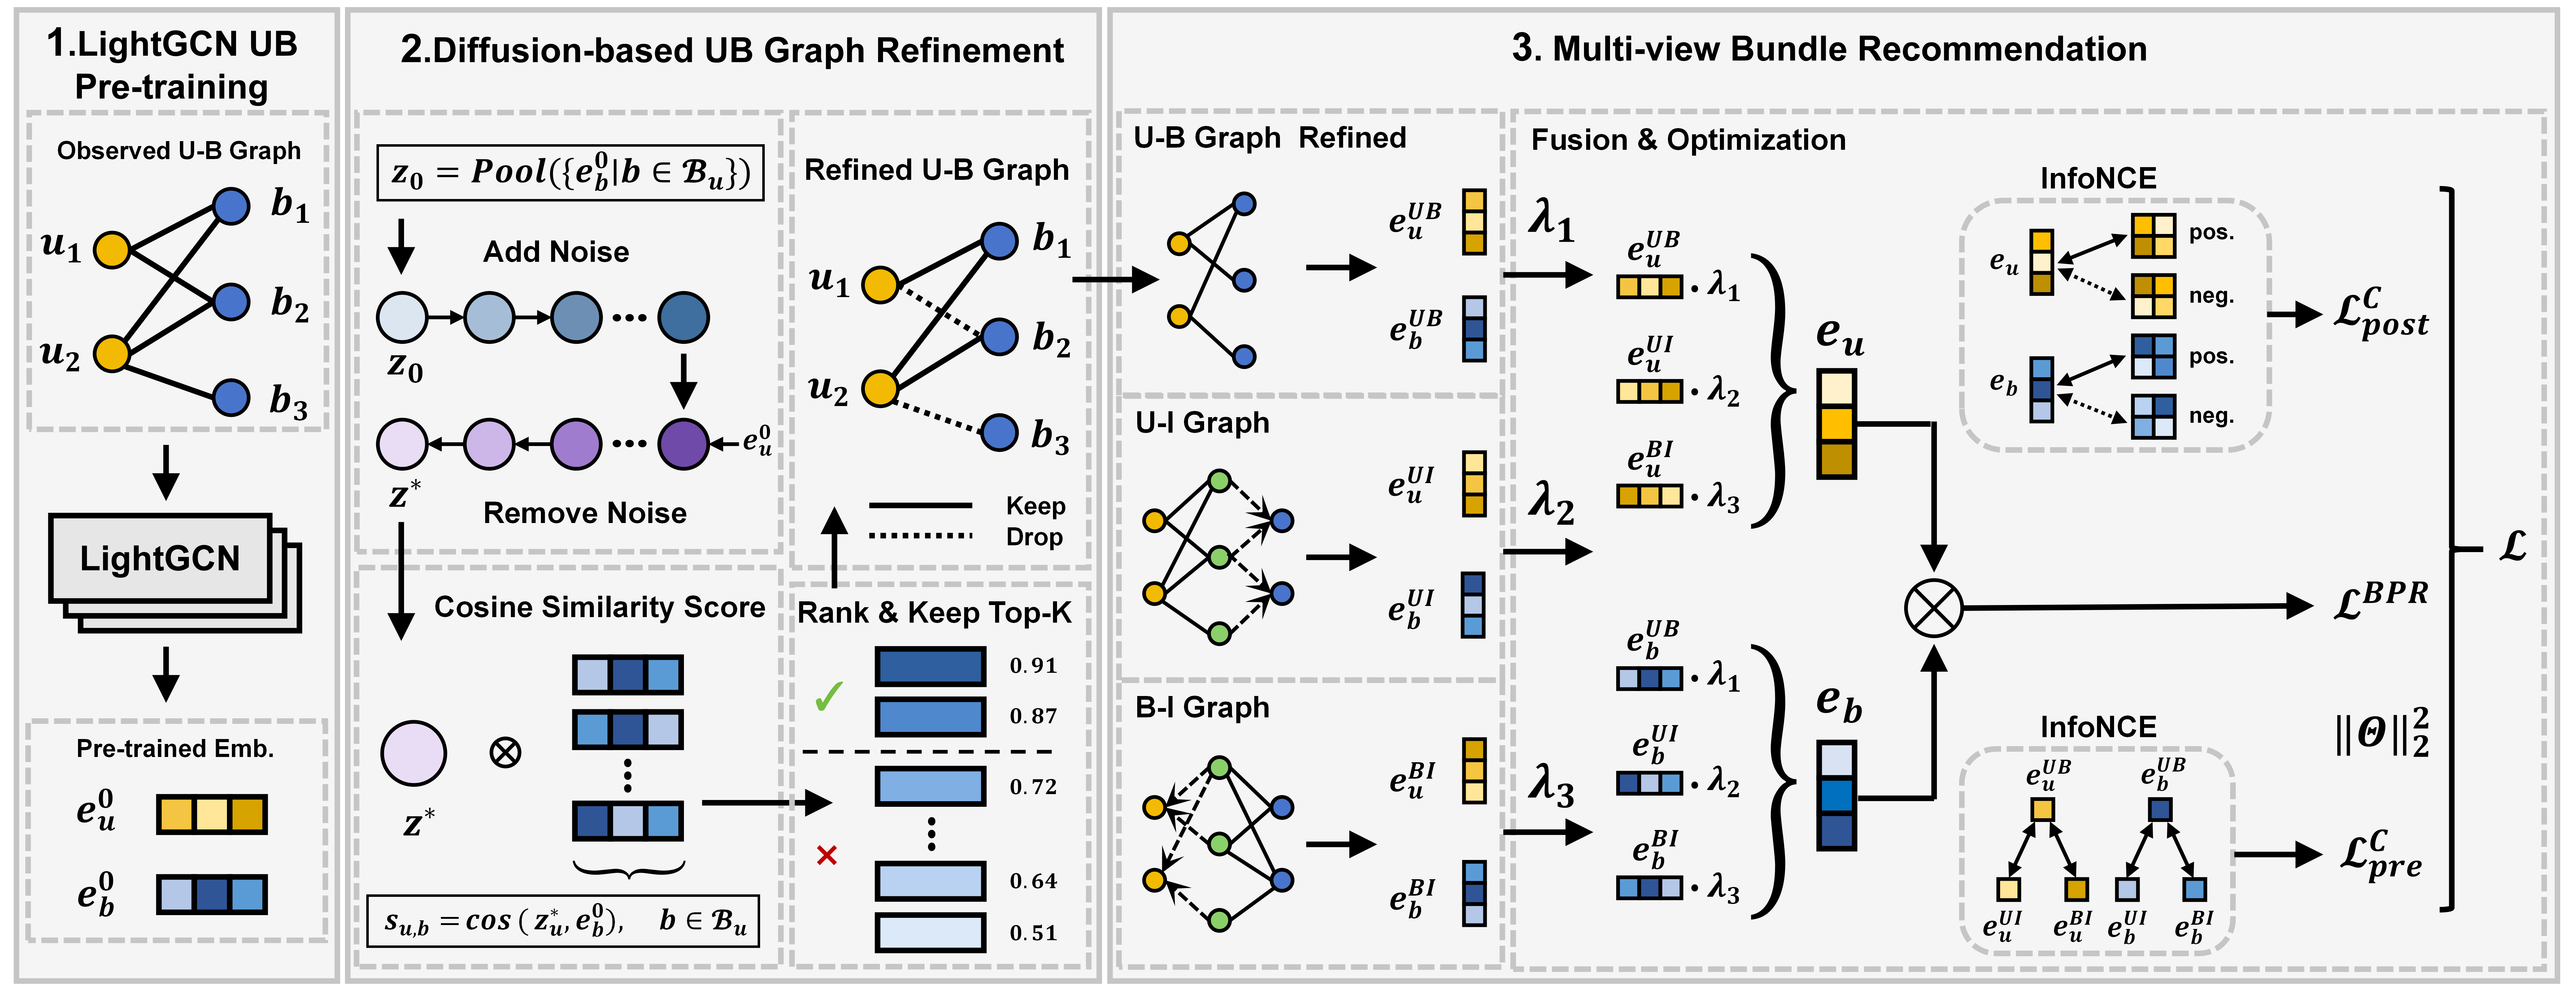
\includegraphics[width=0.98\textwidth]
    {Figures/digo_framework.png}
    \caption{Overall framework of DiGO, comprising (1) user–bundle pretraining, (2) diffusion-driven graph optimization for reconstructing the observed user–bundle graph, and (3) multi-view recommendation using the reconstructed user–bundle view as the anchor for pre-fusion cross-view contrastive learning.}
    \label{fig:framework}
\end{figure*}

\textbf{Challenge 2: Sparse user--bundle implicit feedback.}
User--bundle feedback is substantially sparser than user--item
interactions, providing limited bundle-level supervision.
Although user--item and bundle--item relations offer rich
auxiliary signals, final-stage fusion alone may not fully align
them with user--bundle preference learning. Therefore, effectively
leveraging auxiliary views while preserving consistency with
direct bundle preferences remains challenging.

To address these challenges, we propose DiGO, a diffusion-driven
graph optimization framework for bundle recommendation. DiGO
first aggregates pretrained representations of each user's
historical bundles and conditions a diffusion process on the
pretrained user representation to model the user's overall bundle
preference. The resulting preference representation is then used
to score observed user--bundle interactions, retain more reliable
connections, and reconstruct the graph without introducing new
edges. Finally, DiGO uses representations from the reconstructed
user--bundle graph as anchors to align the user--item and
bundle--item views before fusion, thereby supplementing sparse
supervision. Figure~\ref{fig:framework} illustrates the overall
framework.



The main contributions of this work are summarized as follows:

\begin{itemize}
    \item We propose DiGO, a diffusion-driven graph optimization
    framework that models users' overall bundle preferences
    through conditional diffusion and uses them to re-evaluate
    observed interactions and reconstruct the user--bundle graph.

    \item We use representations learned from the reconstructed
    user--bundle graph as anchors to align the two auxiliary views
    before view fusion, thereby supplementing sparse user--bundle
    supervision.

    \item Experiments on three public datasets show that DiGO
    outperforms existing methods across all evaluation metrics,
    achieving a maximum relative improvement of 10\%. Ablation
    and further analyses also validate the effectiveness of the
    two key designs.
\end{itemize}
\section{Related Work}

\subsection{Bundle Recommendation}

Early bundle recommendation methods primarily relied on
user--bundle interactions and employed collaborative filtering,
matrix factorization, or neural models to learn user and bundle
representations~\cite{earlybundle1,earlybundle2}. Subsequent
graph-based methods further modeled user--bundle, user--item, and
bundle--item relations to capture high-order collaborative
information at both the bundle and item
levels~\cite{bgcn,graphbundle1}.

Recent studies have increasingly focused on multi-view
representation learning and cross-view collaboration. For
example, MIDGN introduces intent disentanglement, CrossCBR
employs cross-view contrastive learning, BundleGT uses graph
Transformers to model structural information, and MultiCBR
learns unified representations through three-view fusion and
contrastive learning~\cite{midgn,crosscbr,bundlegt,ma2024multicbr}.
These methods mainly improve the encoding, fusion, or alignment
of multiple views, while typically using the observed
user--bundle graph directly. In contrast, DiGO re-evaluates
observed user--bundle interactions before multi-view learning and
reconstructs the user--bundle graph accordingly.


\subsection{Diffusion Models for Recommendation}

Diffusion models exhibit strong distribution modeling
capabilities by progressively perturbing data and learning the
corresponding reverse process. In recent years, they have been
applied to collaborative filtering, sequential recommendation,
and knowledge graph recommendation to model user preferences,
recover interaction signals, or enhance recommendation
representations~\cite{diffrec,diffurec,diffkg}.

Diffusion models have also been introduced into bundle
recommendation. RDiffBR addresses dynamic bundle--item relations
by applying residual diffusion to item-level bundle
representations, enabling the model to adapt to changes in bundle
composition~\cite{rdiffbr}. DCBR applies conditional diffusion to
user--bundle interaction data and combines it with multi-view
contrastive learning~\cite{dcbr}. Unlike these methods, DiGO
aggregates the pretrained representations of bundles in each
user's interaction history and conditions the diffusion process
on the pretrained user representation to model the user's overall
bundle preference. The resulting preference representation is
then used to evaluate observed user--bundle interactions and
reconstruct the user--bundle graph for subsequent multi-view
representation learning.



\section{Methodology}

\subsection{Problem Formulation}

Let
$\mathcal U=\{u_1,u_2,\ldots,u_M\}$,
$\mathcal B=\{b_1,b_2,\ldots,b_N\}$, and
$\mathcal I=\{i_1,i_2,\ldots,i_O\}$
denote the sets of users, bundles, and items, respectively, where
$M$, $N$, and $O$ are the corresponding set sizes. We use a
user--bundle interaction matrix
$\mathbf X\in\{0,1\}^{M\times N}$, a user--item interaction
matrix $\mathbf Y\in\{0,1\}^{M\times O}$, and a bundle--item
affiliation matrix $\mathbf Z\in\{0,1\}^{N\times O}$.
Specifically, $x_{ub}=1$ and $y_{ui}=1$ indicate that user $u$
has interacted with bundle $b$ and item $i$, respectively, while
$z_{bi}=1$ indicates that item $i$ belongs to bundle $b$.

Given $\mathbf X$, $\mathbf Y$, and $\mathbf Z$, the goal of
bundle recommendation is to predict the preference score
$y^*_{u,b}$ for each unobserved user--bundle pair.


\subsection{Framework Overview}

As illustrated in Figure~\ref{fig:framework}, DiGO first models
each user's overall bundle preference using pretrained
representations and reconstructs the original user--bundle matrix
$\mathbf X$ as $\widetilde{\mathbf X}$. It then learns user and
bundle representations from three views based on
$\widetilde{\mathbf X}$, $\mathbf Y$, and $\mathbf Z$. Before
fusing the three views, DiGO performs cross-view alignment using
the user--bundle view as the anchor and finally predicts user
preferences from the fused representations.


\subsection{Diffusion-Driven Graph Optimization}

\subsubsection{Preference Representation Construction}

We first pretrain LightGCN~\cite{he2020lightgcn} on the original
user--bundle interactions to obtain pretrained representations
$\bar{\mathbf e}_u$ and $\bar{\mathbf e}_b$ for user $u$ and
bundle $b$, respectively. The pretraining model is optimized with
the BPR objective, and the resulting representations remain fixed
during subsequent graph optimization.

Let
$\mathcal N_u^{UB}
=
\{b\in\mathcal B\mid x_{ub}=1\}$
denote the set of bundles historically interacted with by user
$u$. We construct the historical bundle representation through
mean pooling:

\begin{equation}
\mathbf p_u^0
=
\frac{1}{|\mathcal N_u^{UB}|}
\sum_{b\in\mathcal N_u^{UB}}
\bar{\mathbf e}_b ,
\tag{1}
\end{equation}

where $\mathbf p_u^0$ summarizes the overall characteristics of
the bundles in the user's interaction history and serves as the
modeling target of the subsequent diffusion process.


\subsubsection{Conditional Diffusion}

Given the number of diffusion steps $T$ and a noise schedule
$\{\beta_t\}_{t=1}^{T}$, we define
$\alpha_t=1-\beta_t$ and
$\bar{\alpha}_t=\prod_{s=1}^{t}\alpha_s$.
At timestep $t$, the forward perturbation of $\mathbf p_u^0$ is
defined as

\begin{equation}
\mathbf p_u^t
=
\sqrt{\bar{\alpha}_t}\mathbf p_u^0
+
\sqrt{1-\bar{\alpha}_t}\boldsymbol{\epsilon},
\qquad
\boldsymbol{\epsilon}
\sim
\mathcal N(\mathbf 0,\mathbf I).
\tag{2}
\end{equation}

We use the pretrained user representation
$\bar{\mathbf e}_u$ as a personalized condition and employ a
conditional denoising network to predict the unperturbed bundle
preference representation:

\begin{equation}
\widehat{\mathbf p}_u^0
=
f_\theta
\left(
\mathbf p_u^t,
\bar{\mathbf e}_u,
t
\right),
\tag{3}
\end{equation}

where $f_\theta$ is an MLP-based conditional denoising network
that integrates the perturbed representation, the user condition,
and the timestep embedding.

During training, we uniformly sample $t$ from
$\{1,\ldots,T\}$ and draw Gaussian noise
$\boldsymbol{\epsilon}$ to construct $\mathbf p_u^t$. The
diffusion module is optimized by reconstructing the
unperturbed historical bundle representation:

\begin{equation}
L^{D}
=
\mathbb E_{\substack{
u\sim\mathcal U^{+},\,
t\sim\operatorname{Unif}\{1,\ldots,T\},\\
\boldsymbol{\epsilon}\sim\mathcal N(\mathbf 0,\mathbf I)
}}
\left[
\left\|
\widehat{\mathbf p}_u^0-\mathbf p_u^0
\right\|_2^2
\right],
\tag{4}
\end{equation}

where
$\mathcal U^{+}
=
\{u\in\mathcal U\mid|\mathcal N_u^{UB}|>0\}$.
This objective encourages the conditional denoising network
to recover the overall representation of the bundles in the
user's interaction history.


\subsubsection{Interaction Scoring and Graph Reconstruction}

During graph reconstruction, we employ a deterministic iterative
denoising procedure. The historical bundle representation is used
as the initial state, and the conditional denoising network is
repeatedly applied in reverse timestep order:

\begin{equation}
\begin{aligned}
\widetilde{\mathbf p}_u^{T}
&=
\mathbf p_u^0,
\\
\widetilde{\mathbf p}_u^{t-1}
&=
f_\theta
\left(
\widetilde{\mathbf p}_u^{t},
\bar{\mathbf e}_u,
t
\right),
\\
\mathbf p_u^{*}
&=
\widetilde{\mathbf p}_u^{0},
\end{aligned}
\qquad
t=T,T-1,\ldots,1.
\tag{5}
\end{equation}

Here, $\mathbf p_u^{*}$ denotes the resulting overall bundle
preference representation of user $u$.

We then compute preference-matching scores only for the user's
observed interactions and retain at most the top-$\kappa$
bundles:

\begin{equation}
\begin{aligned}
s_{u,b}
&=
\cos
\left(
\mathbf p_u^{*},
\bar{\mathbf e}_b
\right),
\qquad
b\in\mathcal N_u^{UB},
\\
\widetilde{\mathcal N}_u^{UB}
&=
\operatorname{TopK}_{b\in\mathcal N_u^{UB}}
\left(
s_{u,b},
\kappa
\right),
\\
\widetilde{x}_{ub}
&=
\mathbb I
\left[
b\in\widetilde{\mathcal N}_u^{UB}
\right].
\end{aligned}
\tag{6}
\end{equation}

Here, $\kappa$ is the maximum number of interactions retained for
each user, and $\mathbb I[\cdot]$ is the indicator function. All
$\widetilde{x}_{ub}$ form the reconstructed user--bundle matrix
$\widetilde{\mathbf X}$. Since
$\widetilde{\mathcal N}_u^{UB}
\subseteq
\mathcal N_u^{UB}$,
DiGO only re-evaluates and filters observed user--bundle
interactions without introducing unobserved connections.


\subsection{Multi-View Representation Learning}

Based on $\widetilde{\mathbf X}$, $\mathbf Y$, and $\mathbf Z$,
DiGO learns representations from the user--bundle interaction
view, user--item interaction view, and bundle--item affiliation
view. The three views share the initial trainable user, bundle,
and item representations while employing independent propagation
paths.

Let $\operatorname{LG}(\cdot)$ denote a LightGCN encoder with
neighborhood propagation and layer-wise aggregation. The
representation learning process for the three views is written as

\begin{equation}
\begin{aligned}
\left(
\mathbf E_U^{UB},
\mathbf E_B^{UB}
\right)
&=
\operatorname{LG}
\left(
\widetilde{\mathbf X}
\right),
\\
\left(
\mathbf E_U^{UI},
\mathbf E_I^{UI}
\right)
&=
\operatorname{LG}
\left(
\mathbf Y
\right),
\\
\mathbf e_b^{UI}
&=
\frac{1}{|\mathcal N_b^{BI}|}
\sum_{i\in\mathcal N_b^{BI}}
\mathbf e_i^{UI},
\\
\left(
\mathbf E_B^{BI},
\mathbf E_I^{BI}
\right)
&=
\operatorname{LG}
\left(
\mathbf Z
\right),
\\
\mathbf e_u^{BI}
&=
\frac{1}{|\mathcal N_u^{UI}|}
\sum_{i\in\mathcal N_u^{UI}}
\mathbf e_i^{BI}.
\end{aligned}
\tag{7}
\end{equation}

Here, $\mathcal N_b^{BI}$ denotes the set of items contained in
bundle $b$, while $\mathcal N_u^{UI}$ denotes the set of items
interacted with by user $u$. The UB view directly produces the
user representation $\mathbf e_u^{UB}$ and bundle representation
$\mathbf e_b^{UB}$. In the UI view, item representations are
aggregated according to bundle--item affiliations to obtain
$\mathbf e_b^{UI}$. In the BI view, item representations are
aggregated according to user--item interactions to obtain
$\mathbf e_u^{BI}$. This three-view organization follows the
standard multi-view modeling framework for bundle
recommendation~\cite{ma2024multicbr}.

Consequently, user $u$ obtains three view-specific representations
$\{\mathbf e_u^{UB},\mathbf e_u^{UI},\mathbf e_u^{BI}\}$, while
bundle $b$ obtains
$\{\mathbf e_b^{UB},\mathbf e_b^{UI},\mathbf e_b^{BI}\}$.


\subsection{Cross-View Contrastive Learning}

To exploit the two auxiliary views for supplementing sparse
user--bundle supervision, DiGO uses the representations learned
from the reconstructed user--bundle view as anchors and aligns
them with the user--item and bundle--item representations before
fusing the three views.

For an entity set $\mathcal S$, the contrastive loss between an
anchor view $a$ and an auxiliary view $v$ is defined as

\begin{equation}
\begin{aligned}
\ell_{\tau}
\left(
\mathbf E^{a},
\mathbf E^{v};
\mathcal S
\right)
=
-\frac{1}{|\mathcal S|}
\sum_{x\in\mathcal S}
\log
\frac{
\exp
\left(
\cos(\mathbf e_x^{a},\mathbf e_x^{v})/\tau
\right)
}{
\sum_{x'\in\mathcal S}
\exp
\left(
\cos(\mathbf e_x^{a},\mathbf e_{x'}^{v})/\tau
\right)
}.
\end{aligned}
\tag{8}
\end{equation}

Representations of the same entity across the two views form a
positive pair, while representations of the remaining entities
serve as in-batch negatives.

The pre-fusion cross-view contrastive loss is defined as

\begin{equation}
\begin{aligned}
L^{A}
={}&
\ell_{\tau_a}
\left(
\mathbf E_U^{UB},
\mathbf E_U^{UI};
\mathcal S_U
\right)
+
\ell_{\tau_a}
\left(
\mathbf E_U^{UB},
\mathbf E_U^{BI};
\mathcal S_U
\right)
\\
&+
\ell_{\tau_a}
\left(
\mathbf E_B^{UB},
\mathbf E_B^{UI};
\mathcal S_B
\right)
+
\ell_{\tau_a}
\left(
\mathbf E_B^{UB},
\mathbf E_B^{BI};
\mathcal S_B
\right),
\end{aligned}
\tag{9}
\end{equation}

where $\mathcal S_U$ and $\mathcal S_B$ denote the sets of
unique users and positive bundles in the current batch,
respectively, and $\tau_a$ is the temperature parameter. DiGO
only constructs UB--UI and UB--BI alignment on both the user and
bundle sides, without introducing an additional UI--BI
constraint.


\subsection{Prediction and Model Optimization}

The user and bundle representations from the three views are
fused using view coefficients, and their inner product is used
for preference prediction:

\begin{equation}
\begin{aligned}
\mathbf e_u
&=
\lambda_1\mathbf e_u^{UB}
+
\lambda_2\mathbf e_u^{UI}
+
\lambda_3\mathbf e_u^{BI},
\\
\mathbf e_b
&=
\lambda_1\mathbf e_b^{UB}
+
\lambda_2\mathbf e_b^{UI}
+
\lambda_3\mathbf e_b^{BI},
\\
y^*_{u,b}
&=
\mathbf e_u^\top\mathbf e_b,
\qquad
\lambda_1+\lambda_2+\lambda_3=1.
\end{aligned}
\tag{10}
\end{equation}

DiGO also retains post-fusion self-supervised contrastive
learning. Let $\mathbf E'_U,\mathbf E''_U$ and
$\mathbf E'_B,\mathbf E''_B$ denote the user and bundle
representations generated by two independent representation
perturbations, respectively. The post-fusion contrastive loss is

\begin{equation}
L^{C}
=
\frac{1}{2}
\left[
\ell_{\tau_c}
\left(
\mathbf E'_U,
\mathbf E''_U;
\mathcal S_U
\right)
+
\ell_{\tau_c}
\left(
\mathbf E'_B,
\mathbf E''_B;
\mathcal S_B
\right)
\right],
\tag{11}
\end{equation}

where $\tau_c$ is the temperature parameter for post-fusion
contrastive learning.

For each training triplet $(u,b,b')$, where $x_{ub}=1$ and
$x_{ub'}=0$, the recommendation loss and the overall objective
of the multi-view recommendation model are defined as

\begin{equation}
\begin{aligned}
L^{BPR}
&=
\sum_{(u,b,b')}
-\ln
\sigma
\left(
y^*_{u,b}
-
y^*_{u,b'}
\right),
\\
L^{R}
&=
L^{BPR}
+
\beta_1L^{C}
+
\beta_2L^{A}
+
\beta_3
\left\|
\Theta
\right\|_2^2,
\end{aligned}
\tag{12}
\end{equation}

where $\Theta$ denotes the trainable parameters of the multi-view
recommendation model, and $\beta_1$, $\beta_2$, and $\beta_3$
control the contributions of the post-fusion contrastive loss,
the pre-fusion cross-view contrastive loss, and the regularization
term, respectively.

During training, DiGO first optimizes the diffusion module with
$L^D$ and reconstructs $\widetilde{\mathbf X}$. It then uses
$\widetilde{\mathbf X}$, $\mathbf Y$, and $\mathbf Z$ as inputs
and optimizes the multi-view recommendation model with $L^R$.


\subsection{Complexity Analysis}

Let $d$, $K$, and $Q$ denote the embedding dimension, the
number of graph propagation layers, and the number of
recommendation mini-batches per epoch, respectively. Let
$C_f=\mathcal O(d^2)$ denote the cost of one forward pass
through the fixed-depth denoising MLP. We use
$\mathcal E_{UB}$, $\mathcal E_{UI}$, and $\mathcal E_{BI}$
to denote the edge sets of the three original graphs, and
$\widetilde{\mathcal E}_{UB}$ for the reconstructed UB graph.
The graph propagation in offline LightGCN pretraining requires
$\mathcal O(K|\mathcal E_{UB}|d)$ per pass. During each
training epoch, the time complexity of DiGO is
\[
\begin{aligned}
\mathcal O\big(&
(T+1)|\mathcal U^+|C_f
+|\mathcal E_{UB}|(d+\log\kappa) \\
&+QKd\big(
|\widetilde{\mathcal E}_{UB}|
+|\mathcal E_{UI}|
+|\mathcal E_{BI}|
\big) \\
&+Q(B_U^2+B_B^2)d
\big),
\end{aligned}
\]
where $B_U$ and $B_B$ are the numbers of unique users and
bundles in a mini-batch. The first two terms jointly account
for diffusion learning and graph reconstruction, while the
remaining terms correspond to multi-view graph propagation
and contrastive learning. Since
$|\widetilde{\mathcal E}_{UB}|\leq|\mathcal E_{UB}|$, DiGO
does not increase propagation costs through graph densification
and avoids scoring all $M\times N$ user--bundle pairs. Its
trainable parameter complexity is
$\mathcal O((M+N+O)d+P_f)$, where $P_f$ denotes the number
of parameters in the denoising network.
\section{Experiments}

% =========================================================
% Table 2: Overall results, double-column table
% =========================================================
\begin{table*}[t]
    \centering
    \scriptsize
    \setlength{\tabcolsep}{2.1pt}
    \renewcommand{\arraystretch}{1.06}

    \resizebox{\textwidth}{!}{
    \begin{tabular}{lrrrrrrrrrrrr}
        \toprule
        \multirow{2}{*}{Method}
        & \multicolumn{4}{c}{Youshu}
        & \multicolumn{4}{c}{NetEase}
        & \multicolumn{4}{c}{iFashion} \\
        \cmidrule(lr){2-5}
        \cmidrule(lr){6-9}
        \cmidrule(lr){10-13}
        & R@10 & N@10 & R@20 & N@20
        & R@10 & N@10 & R@20 & N@20
        & R@10 & N@10 & R@20 & N@20 \\
        \midrule

        BGCN
        & -- & -- & 0.2436 & 0.1329
        & -- & -- & 0.0626 & 0.0328
        & -- & -- & 0.0802 & 0.0582 \\

        MIDGN
        & -- & -- & 0.2682 & 0.1527
        & -- & -- & 0.0678 & 0.0343
        & -- & -- & 0.0856 & 0.0473 \\

        CrossCBR
        & -- & -- & 0.2823 & 0.1670
        & -- & -- & 0.0844 & 0.0458
        & -- & -- & 0.1132 & 0.0872 \\

        BundleGT
        & -- & --
        & \underline{0.2905}
        & \underline{0.1737}
        & -- & -- & 0.0903 & 0.0478
        & -- & -- & 0.1263 & 0.0969 \\

        MultiCBR
        & 0.1995 & 0.1439 & 0.2847 & 0.1681
        & 0.0578 & 0.0389 & 0.0901 & 0.0491
        & \underline{0.1057}
        & \underline{0.1028}
        & \underline{0.1494}
        & \underline{0.1203} \\

        EBRec
        & 0.1984 & 0.1425 & 0.2797 & 0.1659
        & 0.0559 & 0.0376 & 0.0881 & 0.0477
        & 0.0909 & 0.0874 & 0.1327 & 0.1044 \\

        EpicCBR
        & \underline{0.1999}
        & \underline{0.1443}
        & 0.2835 & 0.1682
        & \underline{0.0601}
        & \underline{0.0397}
        & \underline{0.0926}
        & \underline{0.0503}
        & 0.1049 & 0.1022 & 0.1467 & 0.1190 \\

        \textbf{DiGO}
        & \textbf{0.2053}
        & \textbf{0.1482}
        & \textbf{0.2919}
        & \textbf{0.1759}
        & \textbf{0.0617}
        & \textbf{0.0411}
        & \textbf{0.0955}
        & \textbf{0.0511}
        & \textbf{0.1144}
        & \textbf{0.1146}
        & \textbf{0.1568}
        & \textbf{0.1315} \\

        \midrule
        \textbf{Improv.}
        & \textbf{2.70\%}
        & \textbf{2.70\%}
        & \textbf{0.48\%}
        & \textbf{1.27\%}
        & \textbf{2.66\%}
        & \textbf{3.53\%}
        & \textbf{3.13\%}
        & \textbf{1.59\%}
        & \textbf{8.23\%}
        & \textbf{11.48\%}
        & \textbf{4.95\%}
        & \textbf{9.31\%} \\
        \bottomrule
    \end{tabular}
    }

    \caption{Overall performance comparison on three datasets.
    The best and second-best results are highlighted in bold and
    underlined, respectively.}
    \label{tab:overall}
\end{table*}


% =========================================================
% Table 1: Dataset statistics, single-column table
% =========================================================
\begin{table}[t]
    \centering
    \scriptsize
    \setlength{\tabcolsep}{1.7pt}
    \renewcommand{\arraystretch}{1.05}

    \resizebox{\columnwidth}{!}{
    \begin{tabular}{lrrrrrr}
        \toprule
        Dataset
        & \#Users
        & \#Items
        & \#Bundles
        & \#U--I
        & \#U--B
        & \#Avg. I/B \\
        \midrule
        Youshu
        & 8,039
        & 32,770
        & 4,771
        & 138,515
        & 51,377
        & 37.03 \\
        NetEase
        & 18,528
        & 123,628
        & 22,864
        & 1,128,065
        & 302,303
        & 77.80 \\
        iFashion
        & 53,897
        & 42,563
        & 27,694
        & 2,290,645
        & 1,679,708
        & 3.86 \\
        \bottomrule
    \end{tabular}
    }

    \caption{Statistics of the datasets.}
    \label{tab:datasets}
\end{table}


% =========================================================
% Table 3: Ablation study, single-column table
% =========================================================
\begin{table}[t]
    \centering
    \scriptsize
    \setlength{\tabcolsep}{1.8pt}
    \renewcommand{\arraystretch}{1.05}

    \resizebox{\columnwidth}{!}{
    \begin{tabular}{lrrrrrr}
        \toprule
        \multirow{2}{*}{Variant}
        & \multicolumn{2}{c}{Youshu}
        & \multicolumn{2}{c}{NetEase}
        & \multicolumn{2}{c}{iFashion} \\
        \cmidrule(lr){2-3}
        \cmidrule(lr){4-5}
        \cmidrule(lr){6-7}
        & R@20 & N@20
        & R@20 & N@20
        & R@20 & N@20 \\
        \midrule

        \textbf{DiGO}
        & \textbf{0.2919}
        & \textbf{0.1759}
        & \textbf{0.0955}
        & \textbf{0.0511}
        & \textbf{0.1568}
        & \textbf{0.1315} \\

        w/o Graph Opt.
        & 0.2920 & 0.1734
        & 0.0948 & 0.0509
        & 0.1500 & 0.1245 \\

        w/o All CL
        & 0.2326 & 0.1307
        & 0.0512 & 0.0260
        & 0.0400 & 0.0281 \\

        w/o Pre-fusion CL
        & 0.2901 & 0.1692
        & 0.0906 & 0.0487
        & 0.1558 & 0.1304 \\

        w/o Post-fusion CL
        & 0.2595 & 0.1502
        & 0.0682 & 0.0350
        & 0.0461 & 0.0350 \\
        \bottomrule
    \end{tabular}
    }

    \caption{Component ablation results of DiGO. The complete
    model is highlighted in bold.}
    \label{tab:ablation}
\end{table}


\subsection{Experimental Settings}

\paragraph{Datasets and Evaluation Metrics.}
We conduct experiments on three public bundle recommendation
datasets: Youshu, NetEase, and iFashion, which correspond to
book lists, music playlists, and fashion outfits, respectively.
For a fair comparison, we adopt the same preprocessed datasets
and data splits as CrossCBR and MultiCBR
\cite{crosscbr,ma2024multicbr}, where user--bundle interactions
are divided into training, validation, and test sets with a ratio
of 70\%, 10\%, and 20\%, respectively. The dataset statistics
are summarized in Table~\ref{tab:datasets}.

We adopt Recall@$K$ and NDCG@$K$ as evaluation metrics, where
$K\in\{10,20\}$. Following the full-ranking evaluation protocol,
all candidate bundles are ranked for each user after masking the
bundles observed in the training set. We select the model
achieving the best Top-20 performance on the validation set and
report its performance on the test set.

\paragraph{Baselines.}
We compare DiGO with seven representative bundle recommendation
methods, including BGCN, MIDGN, CrossCBR, BundleGT, MultiCBR,
EBRec, and EpicCBR
\cite{bgcn,midgn,crosscbr,bundlegt,ma2024multicbr,ebrec,epiccbr}.
These methods cover representative techniques such as
graph-based collaborative modeling, intent disentanglement,
cross-view contrastive learning, graph Transformers, and
multi-view representation learning. For MultiCBR, EBRec, and
EpicCBR, we rerun their publicly released implementations under
the same data splits and evaluation protocol and report the
average results over three independent runs. DiGO is evaluated
in the same manner. For the remaining baselines, we use the
results reported in their original papers.

\paragraph{Implementation Details.}
We implement DiGO in PyTorch and train it on a single NVIDIA
GeForce RTX 3090 GPU. User, bundle, and item embeddings are
initialized with Xavier initialization. The embedding dimension
and the number of graph propagation layers are set to 64 and 2,
respectively. We optimize the model using Adam with a learning
rate of $10^{-3}$ and a batch size of 2048, and sample one
negative bundle for each positive interaction. The diffusion
step $T$ is set to 9, 12, and 12 on Youshu, NetEase, and
iFashion, respectively, while the maximum number of retained
interactions $\kappa$ is set to 7, 13, and 3. The remaining
hyperparameters are tuned according to validation performance.


\subsection{Overall Performance}

Table~\ref{tab:overall} presents the overall performance of DiGO
and the baseline methods on the three datasets.

As shown in Table~\ref{tab:overall}, DiGO achieves the best
performance on all evaluation metrics across the three datasets,
demonstrating its effectiveness in different bundle
recommendation scenarios. On Youshu, DiGO further improves both
Recall and NDCG despite the strong performance of BundleGT and
EpicCBR. On NetEase, DiGO consistently outperforms all baselines
on the four metrics. The improvements are particularly pronounced
on iFashion, where DiGO surpasses the strongest baselines by
8.23\%, 11.48\%, 4.95\%, and 9.31\% in R@10, N@10, R@20, and
N@20, respectively.

Moreover, DiGO consistently outperforms MultiCBR on all three
datasets. MultiCBR already exploits multi-view information
through three-view graph propagation, representation fusion, and
post-fusion contrastive learning. The consistent improvements
achieved by DiGO demonstrate the benefit of further optimizing
the user--bundle graph and aligning the two auxiliary views with
the reconstructed user--bundle view before view fusion.


\subsection{Ablation Study}

To investigate the contribution of each component, we compare
DiGO with four variants. \textbf{w/o Graph Opt.} removes
diffusion-driven graph optimization and directly uses the
original user--bundle graph. \textbf{w/o All CL} removes both the
pre-fusion and post-fusion contrastive objectives.
\textbf{w/o Pre-fusion CL} removes the cross-view contrastive
learning that uses the reconstructed UB view as the anchor.
\textbf{w/o Post-fusion CL} removes the self-supervised
contrastive learning applied after view fusion. The results are
presented in Table~\ref{tab:ablation}.

The contribution of graph optimization varies across datasets.
Removing this component reduces R@20 and N@20 on iFashion from
0.15680 and 0.13150 to 0.14999 and 0.12446, respectively,
resulting in the most noticeable degradation. It also causes
performance drops on NetEase. On Youshu, R@20 remains nearly
unchanged, whereas N@20 decreases. These results indicate that
graph optimization provides dataset-dependent benefits and
contributes most prominently on iFashion.

Removing pre-fusion cross-view contrastive learning also leads
to performance degradation, with more evident changes on Youshu
and NetEase. For example, R@20 and N@20 on NetEase decrease from
0.09550 and 0.05110 to 0.09057 and 0.04873, respectively. This
demonstrates that aligning the UI and BI representations with the
reconstructed UB view before fusion enables the auxiliary
relations to more effectively supplement user--bundle
supervision.

Removing post-fusion contrastive learning causes substantial
performance degradation, while removing both contrastive
objectives leads to a further severe decline. This observation
confirms that post-fusion contrastive learning remains an
important component of the multi-view recommendation backbone.
Meanwhile, the pre-fusion and post-fusion contrastive objectives
operate at different stages---cross-view alignment and
fused-representation optimization---and jointly contribute to
effective multi-view representation learning.


\subsection{In-depth Analysis}

\begin{figure}[t]
    \centering

    % First row
    \begin{minipage}[t]{0.48\columnwidth}
        \centering
        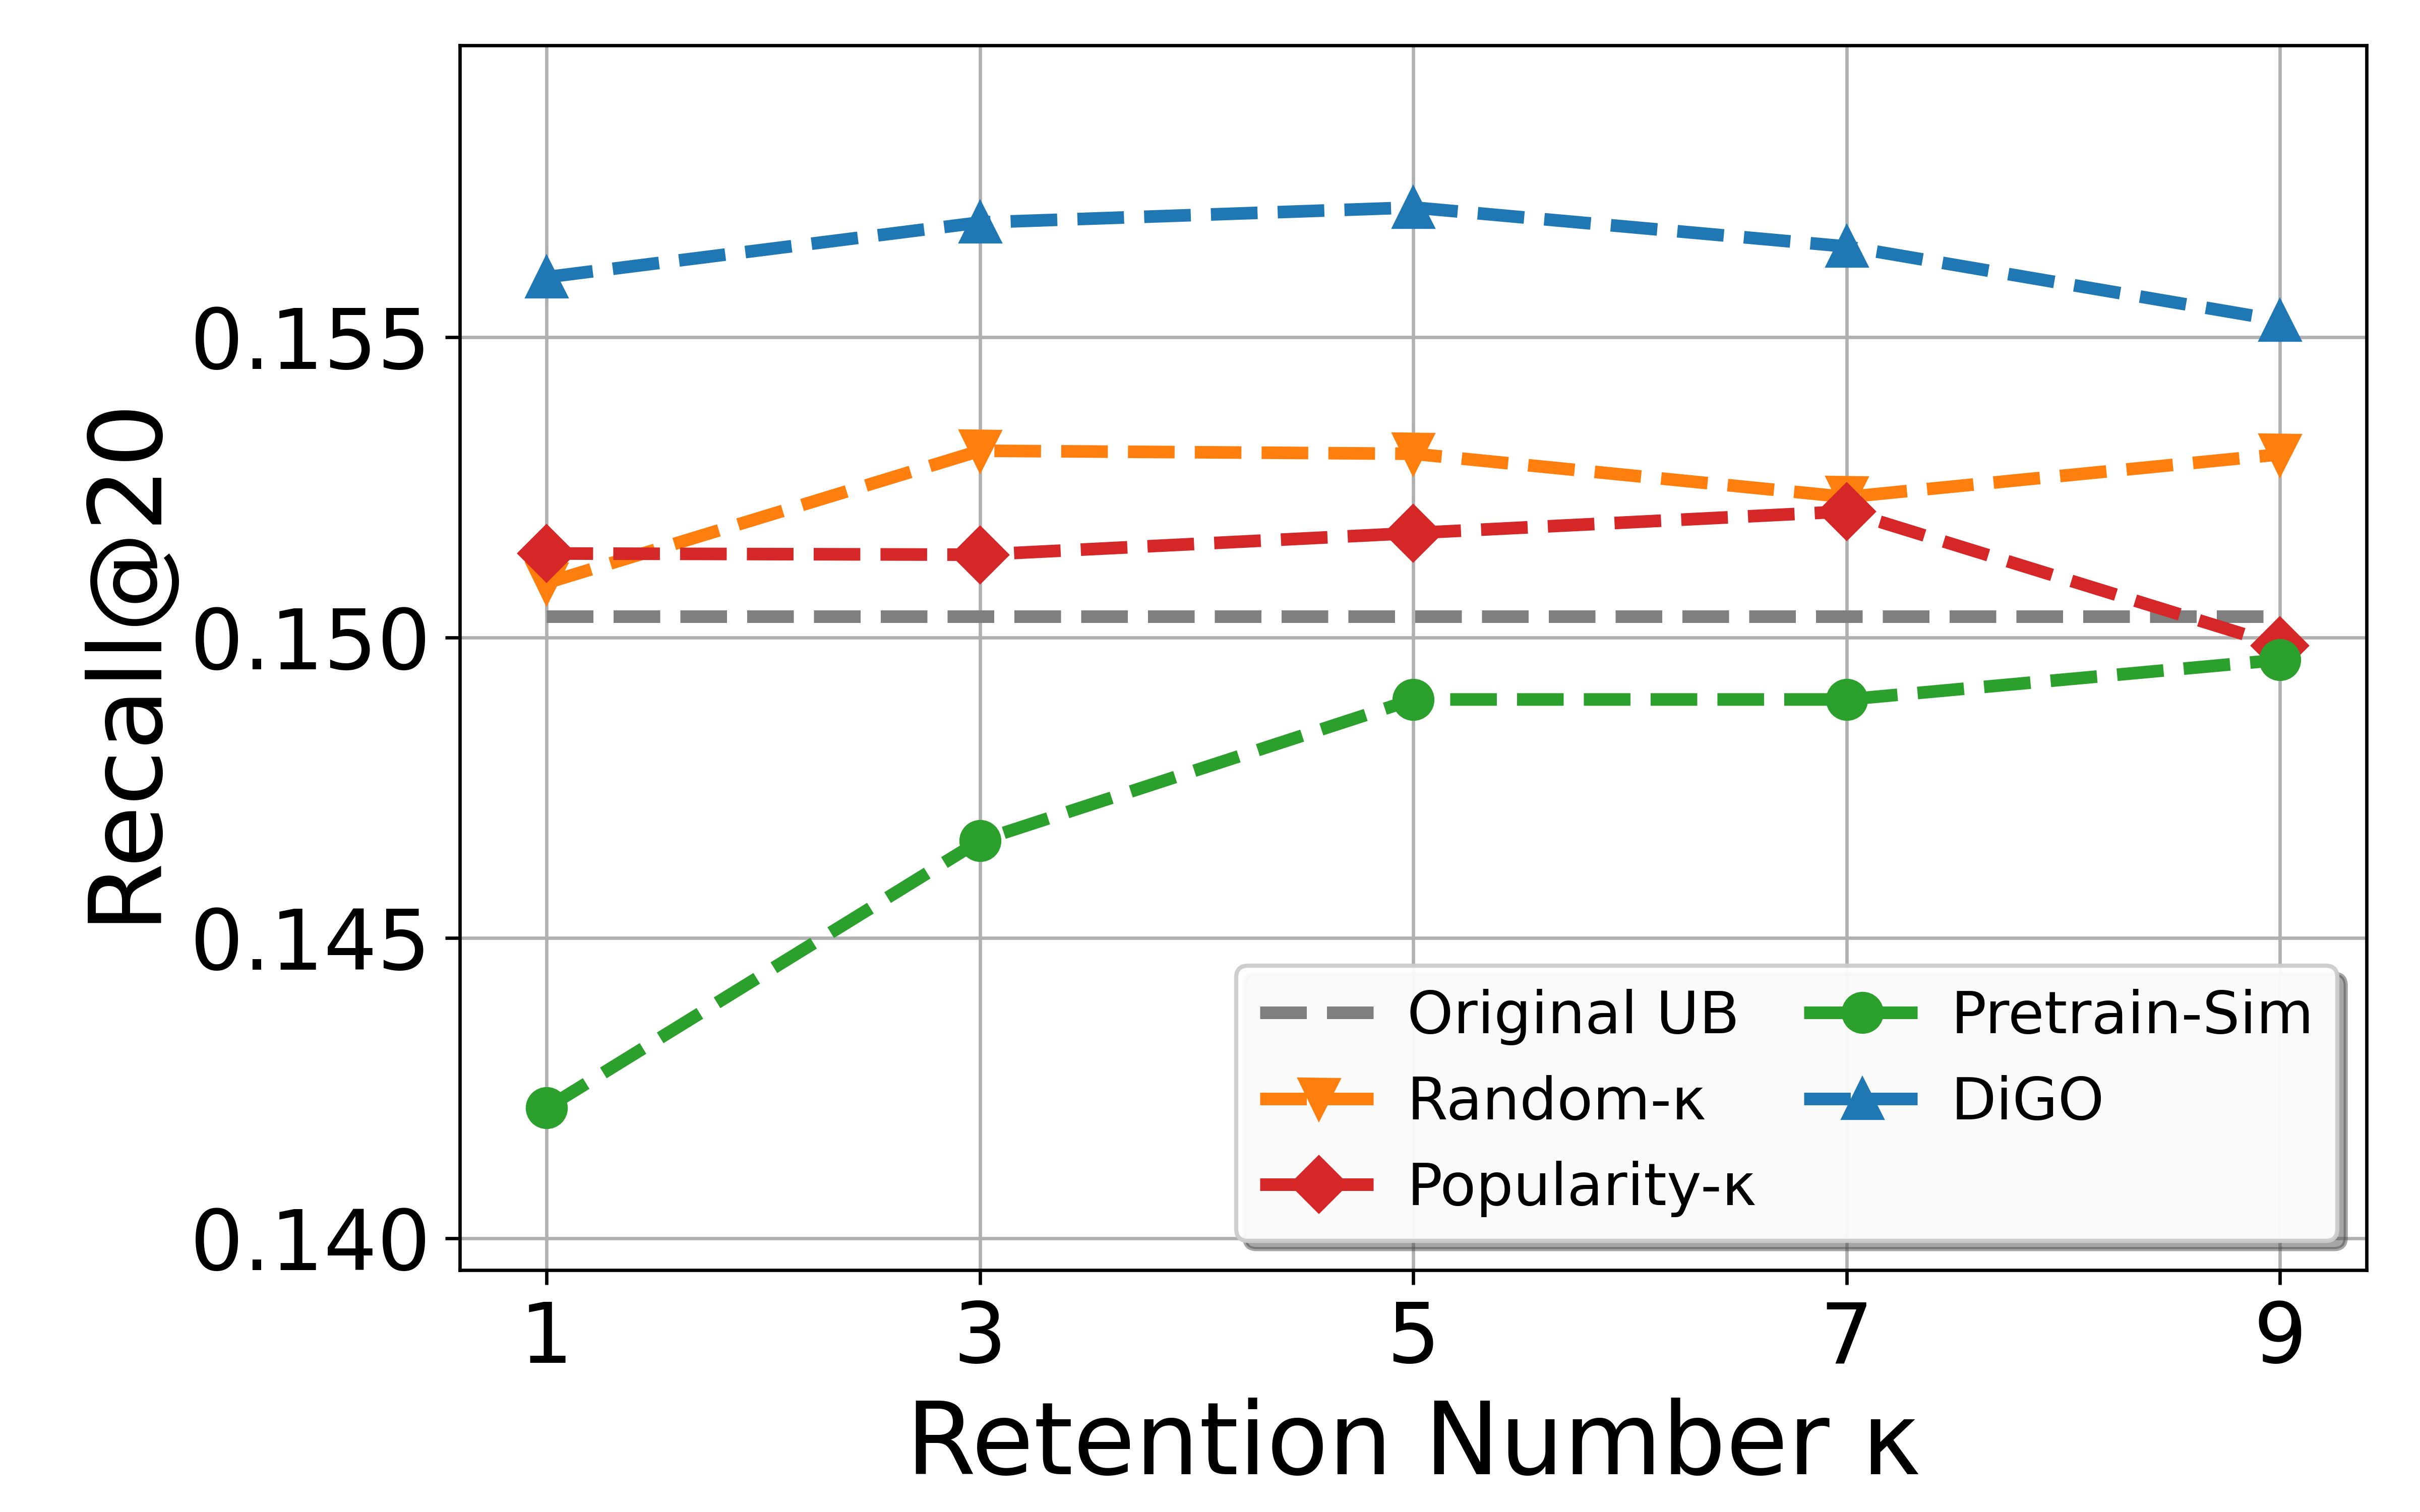
\includegraphics[width=\linewidth]
        {Figures/m1recall20.png}
        \vspace{-2pt}
        \centerline{\small (a)}
    \end{minipage}
    \hfill
    \begin{minipage}[t]{0.48\columnwidth}
        \centering
        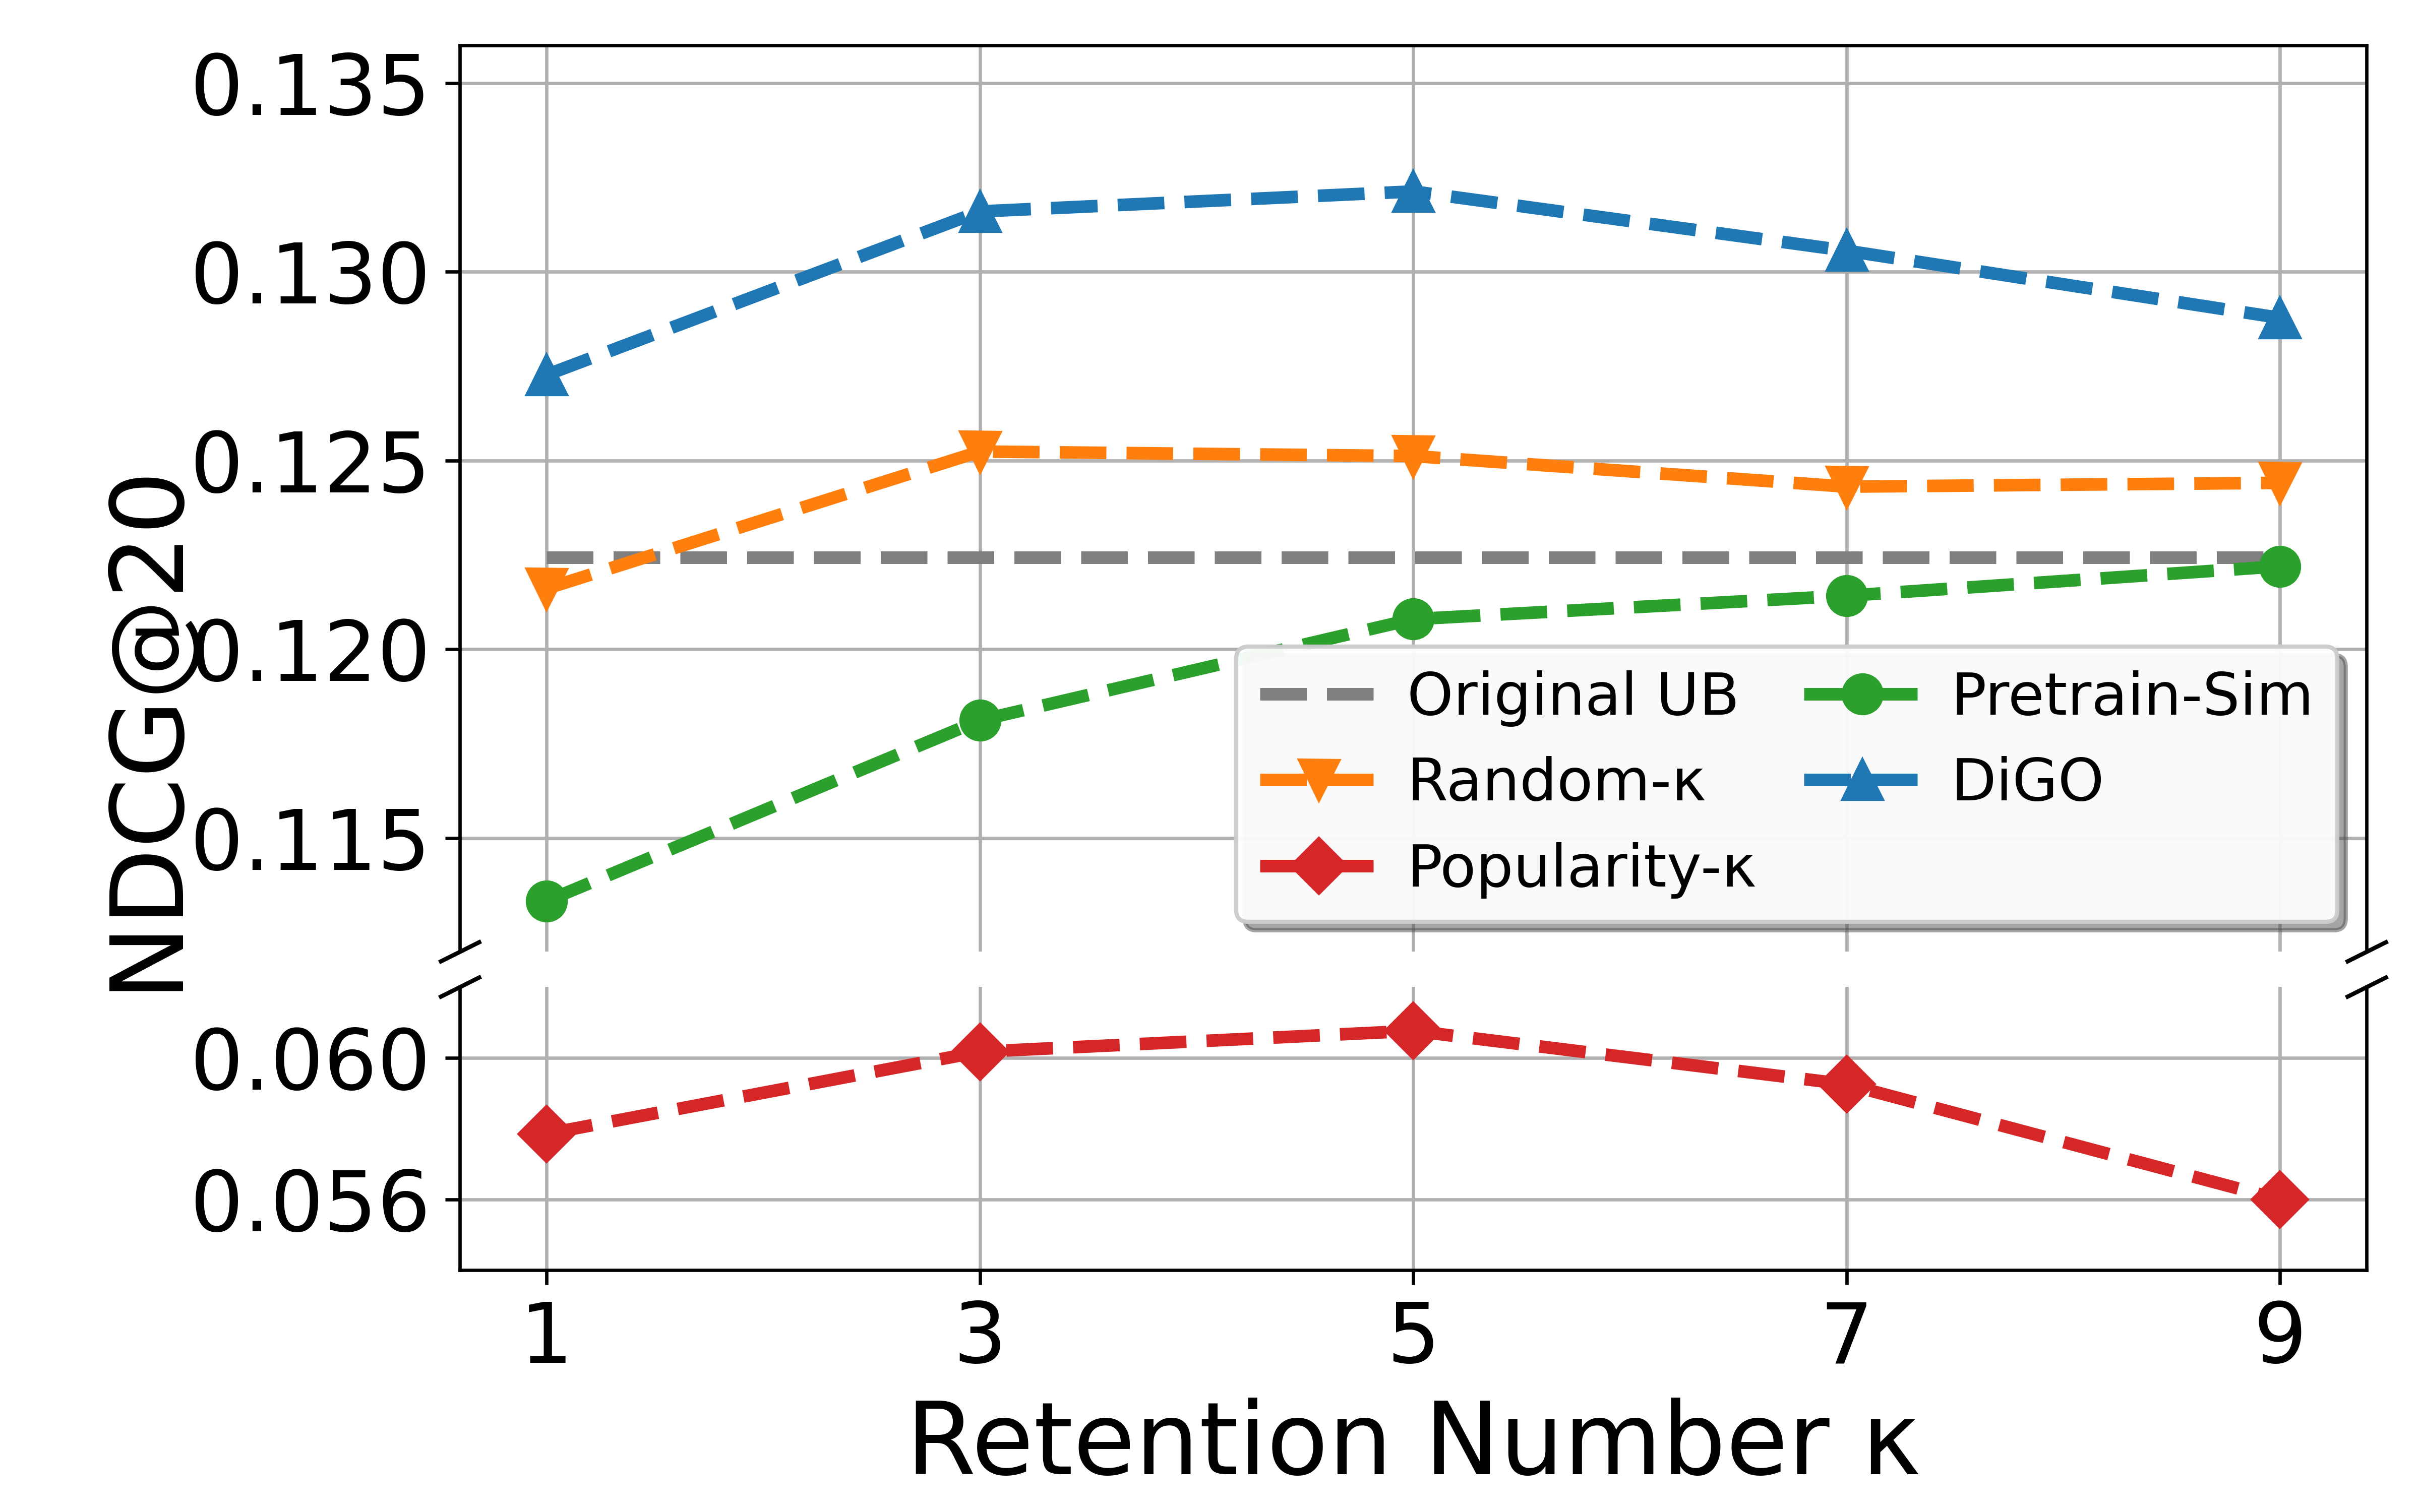
\includegraphics[width=\linewidth]
        {Figures/m1ndcg20.png}
        \vspace{-2pt}
        \centerline{\small (b)}
    \end{minipage}

    \vspace{3pt}

    % Second row
    \begin{minipage}[t]{0.48\columnwidth}
        \centering
        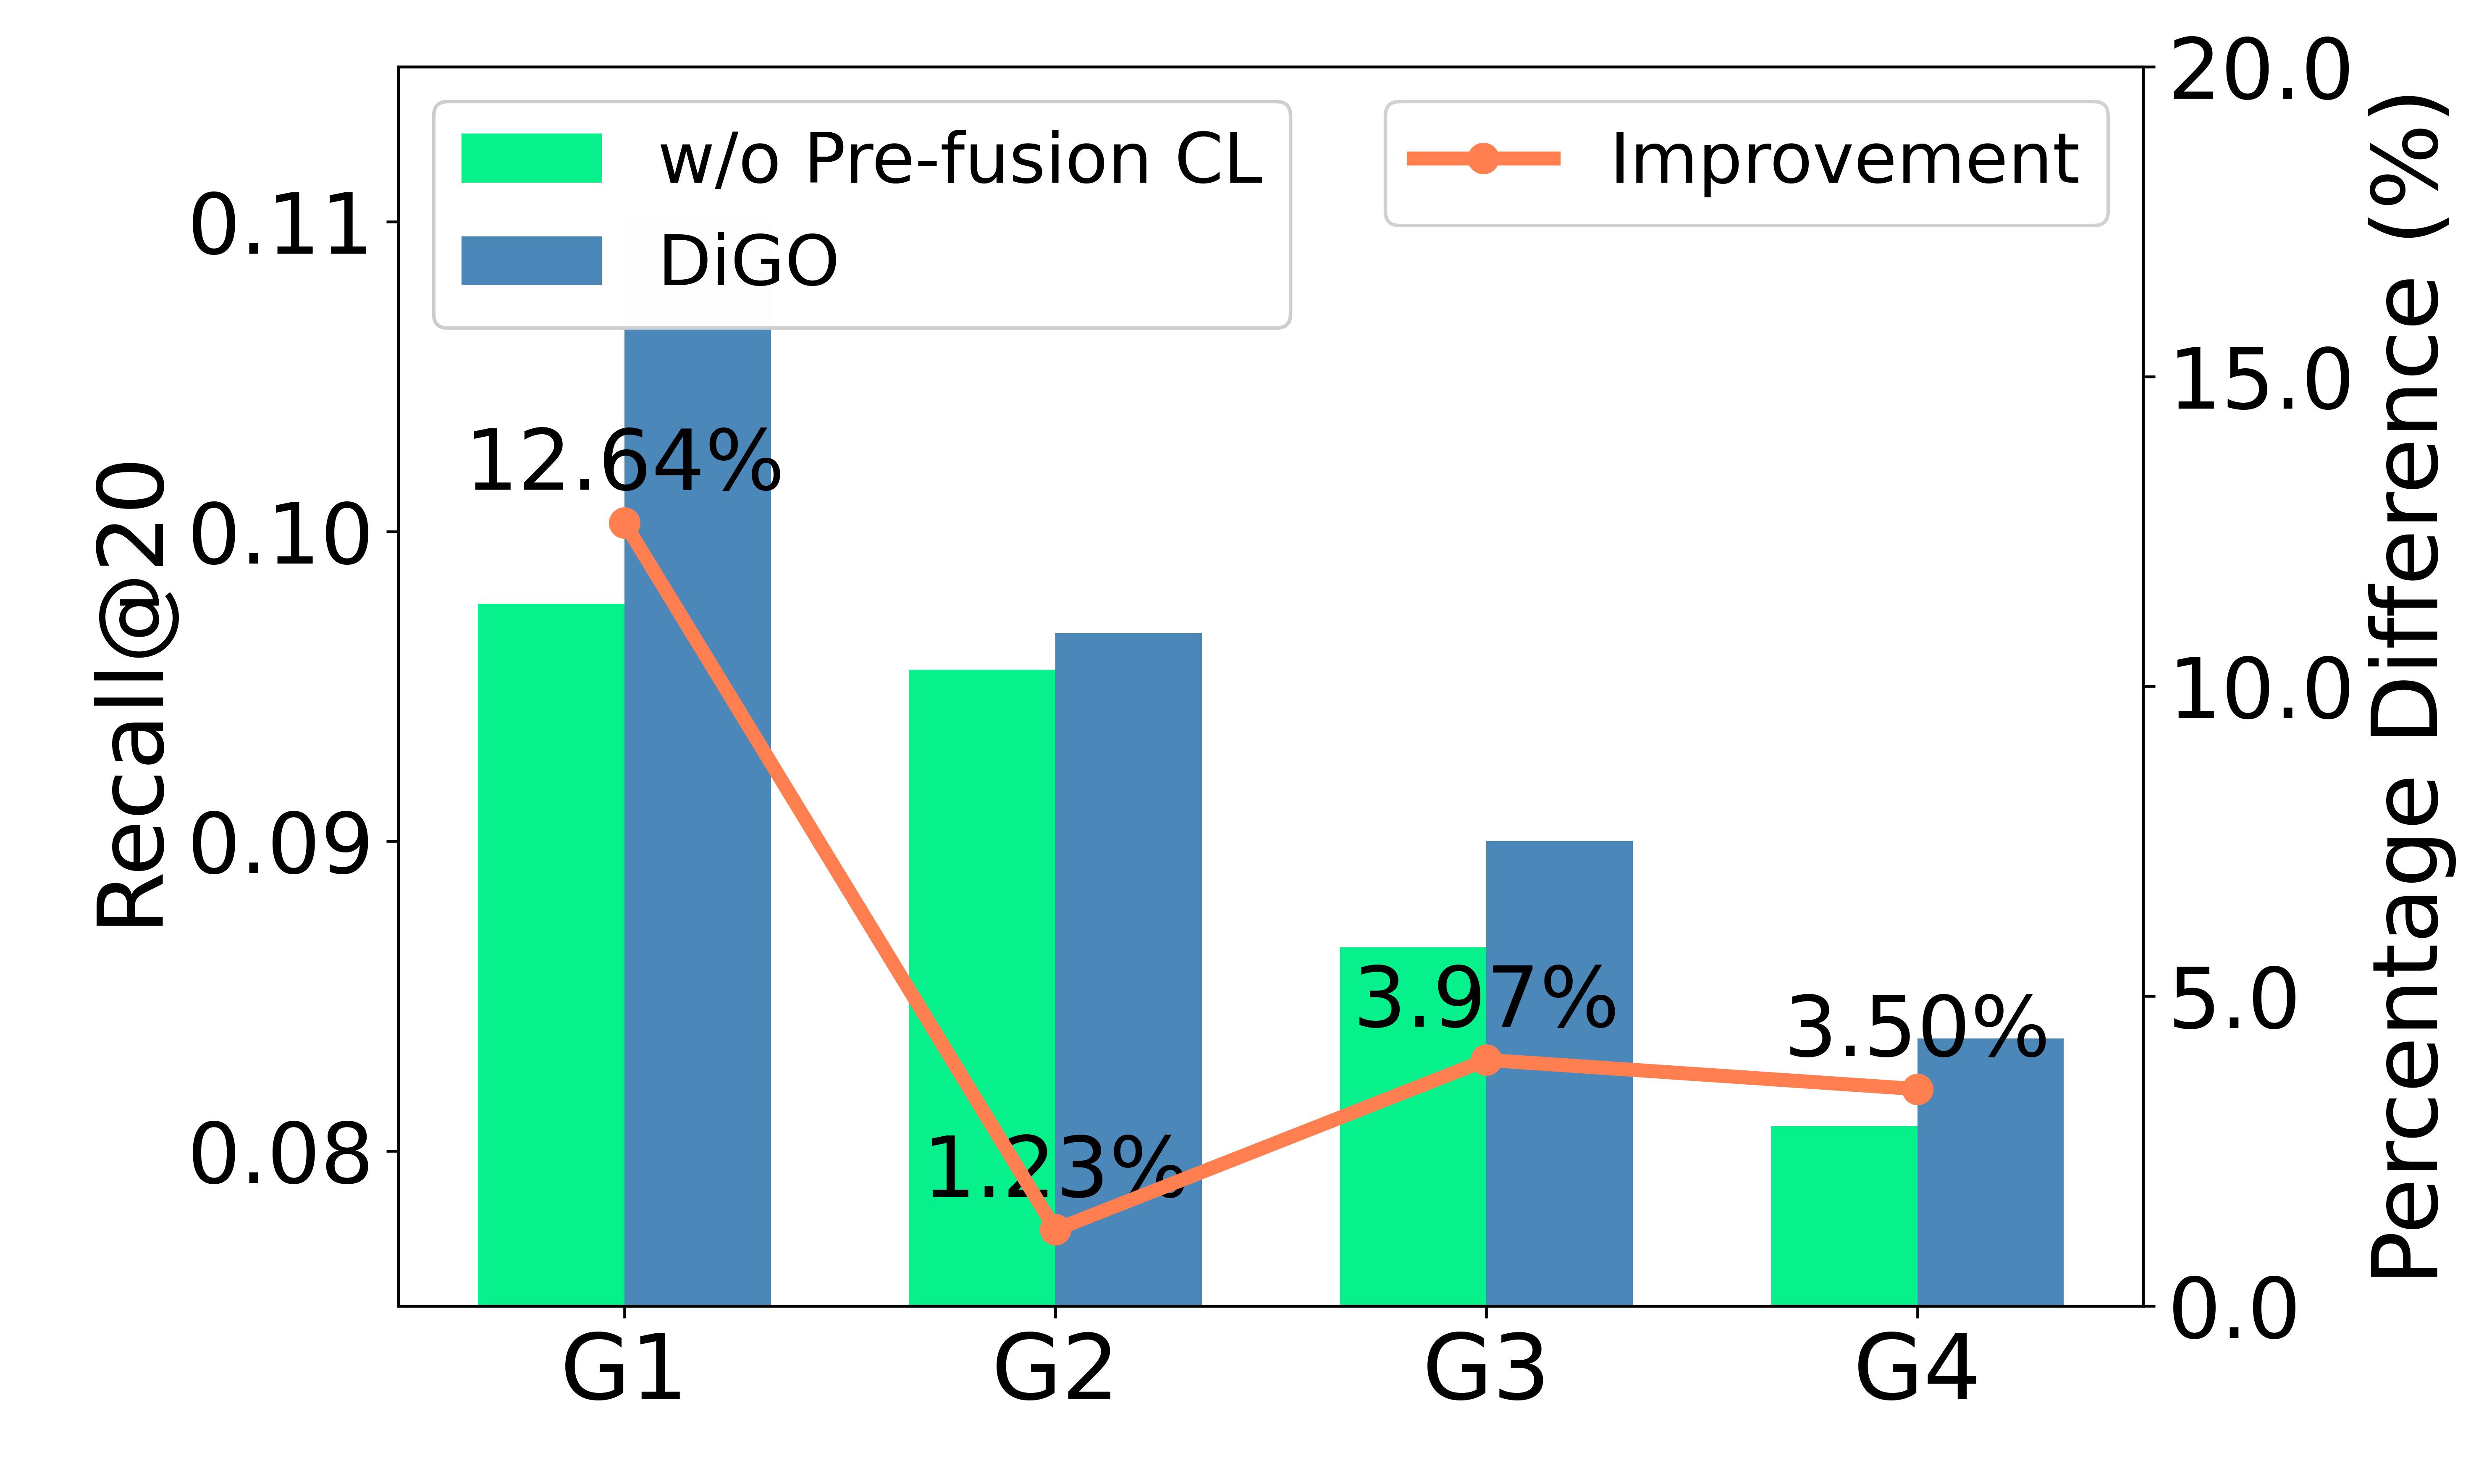
\includegraphics[width=\linewidth]
        {Figures/m2recall20.png}
        \vspace{-2pt}
        \centerline{\small (c)}
    \end{minipage}
    \hfill
    \begin{minipage}[t]{0.48\columnwidth}
        \centering
        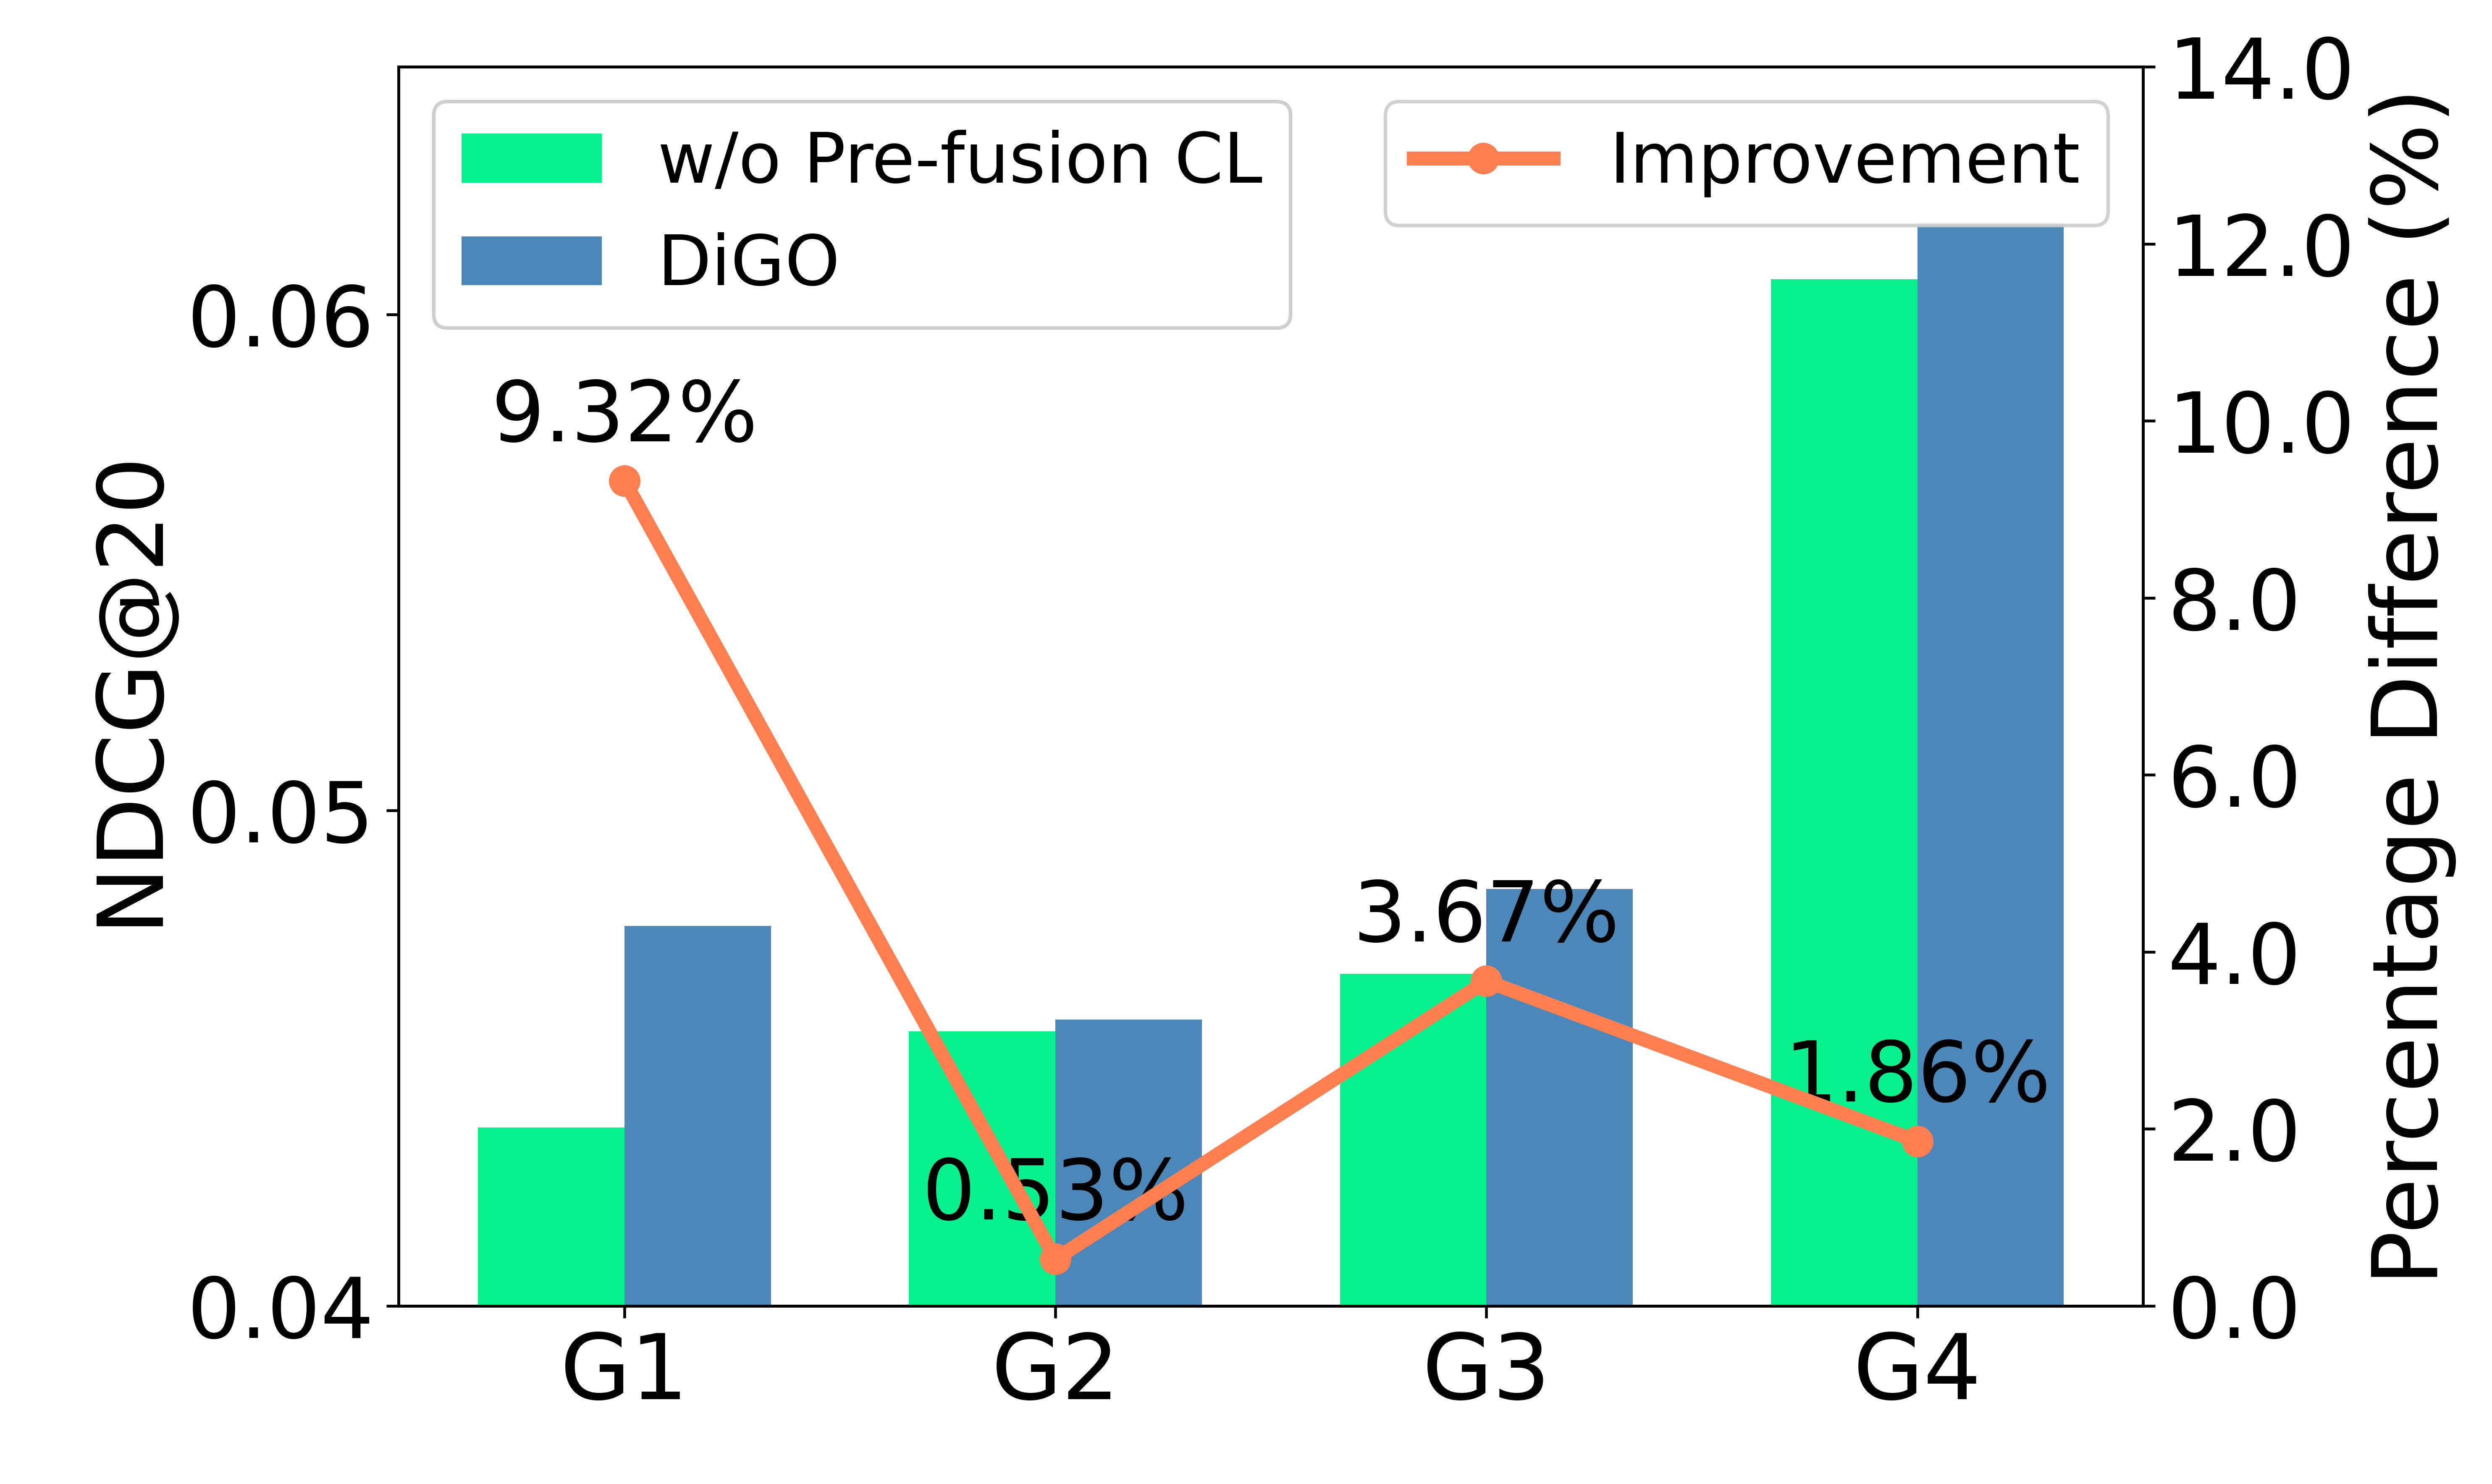
\includegraphics[width=\linewidth]
        {Figures/m2ndcg20.png}
        \vspace{-2pt}
        \centerline{\small (d)}
    \end{minipage}

    \caption{\textbf{In-depth analysis of DiGO.}
    (a)--(b) compare different interaction selection strategies
    on iFashion under varying retention numbers.
    (c)--(d) compare the performance with and without pre-fusion
    cross-view contrastive learning across four user groups on
    NetEase. Users are sorted by their training UB degrees, and
    G1--G4 correspond to $[0,7)$, $[7,8)$, $[8,12)$, and
    $[12,660]$, respectively. Graph optimization is disabled in
    (c)--(d), and the line reports the relative improvement
    introduced by pre-fusion contrastive learning.}
    \label{fig:in-depth-analysis}
\end{figure}


\paragraph{Interaction Selection Strategies.}
To further examine whether diffusion-driven graph optimization
can effectively identify reliable user--bundle interactions, we
compare five graph construction strategies on iFashion.
\textbf{Original UB} directly uses the observed user--bundle
graph without interaction filtering. \textbf{Random-$K$}
randomly retains at most $K$ observed interactions for each user,
while \textbf{Popularity-$K$} selects interactions according to
the global popularity of the corresponding bundles.
\textbf{Pretrain-Sim} ranks observed interactions using the
cosine similarity between pretrained user and bundle
representations. In contrast, \textbf{DiGO} scores each observed
interaction using the overall bundle preference representation
produced by conditional diffusion. All strategies select
connections only from the observed interaction history, and the
results are averaged over multiple independent runs.

As shown in Figure~\ref{fig:in-depth-analysis}(a)--(b), DiGO
consistently achieves the best Recall@20 and NDCG@20 under all
retention settings. Although Random-$K$ occasionally improves
over Original UB, it remains consistently inferior to DiGO,
indicating that the gains cannot be attributed merely to reducing
the number of graph edges. Pretrain-Sim also performs worse than
DiGO, suggesting that directly measuring the similarity between
pretrained user and bundle representations is insufficient to
characterize the overall preference reflected by a user's
interaction history. By modeling historical bundles through
user-conditioned diffusion, DiGO provides a more effective
criterion for re-evaluating observed interactions. Its
performance generally first increases and then decreases as the
retention number grows, reflecting the trade-off between
preserving informative supervision and filtering potentially
unreliable interactions.


\begin{figure*}[t]
    \centering

    \begin{minipage}[t]{0.32\textwidth}
        \centering
        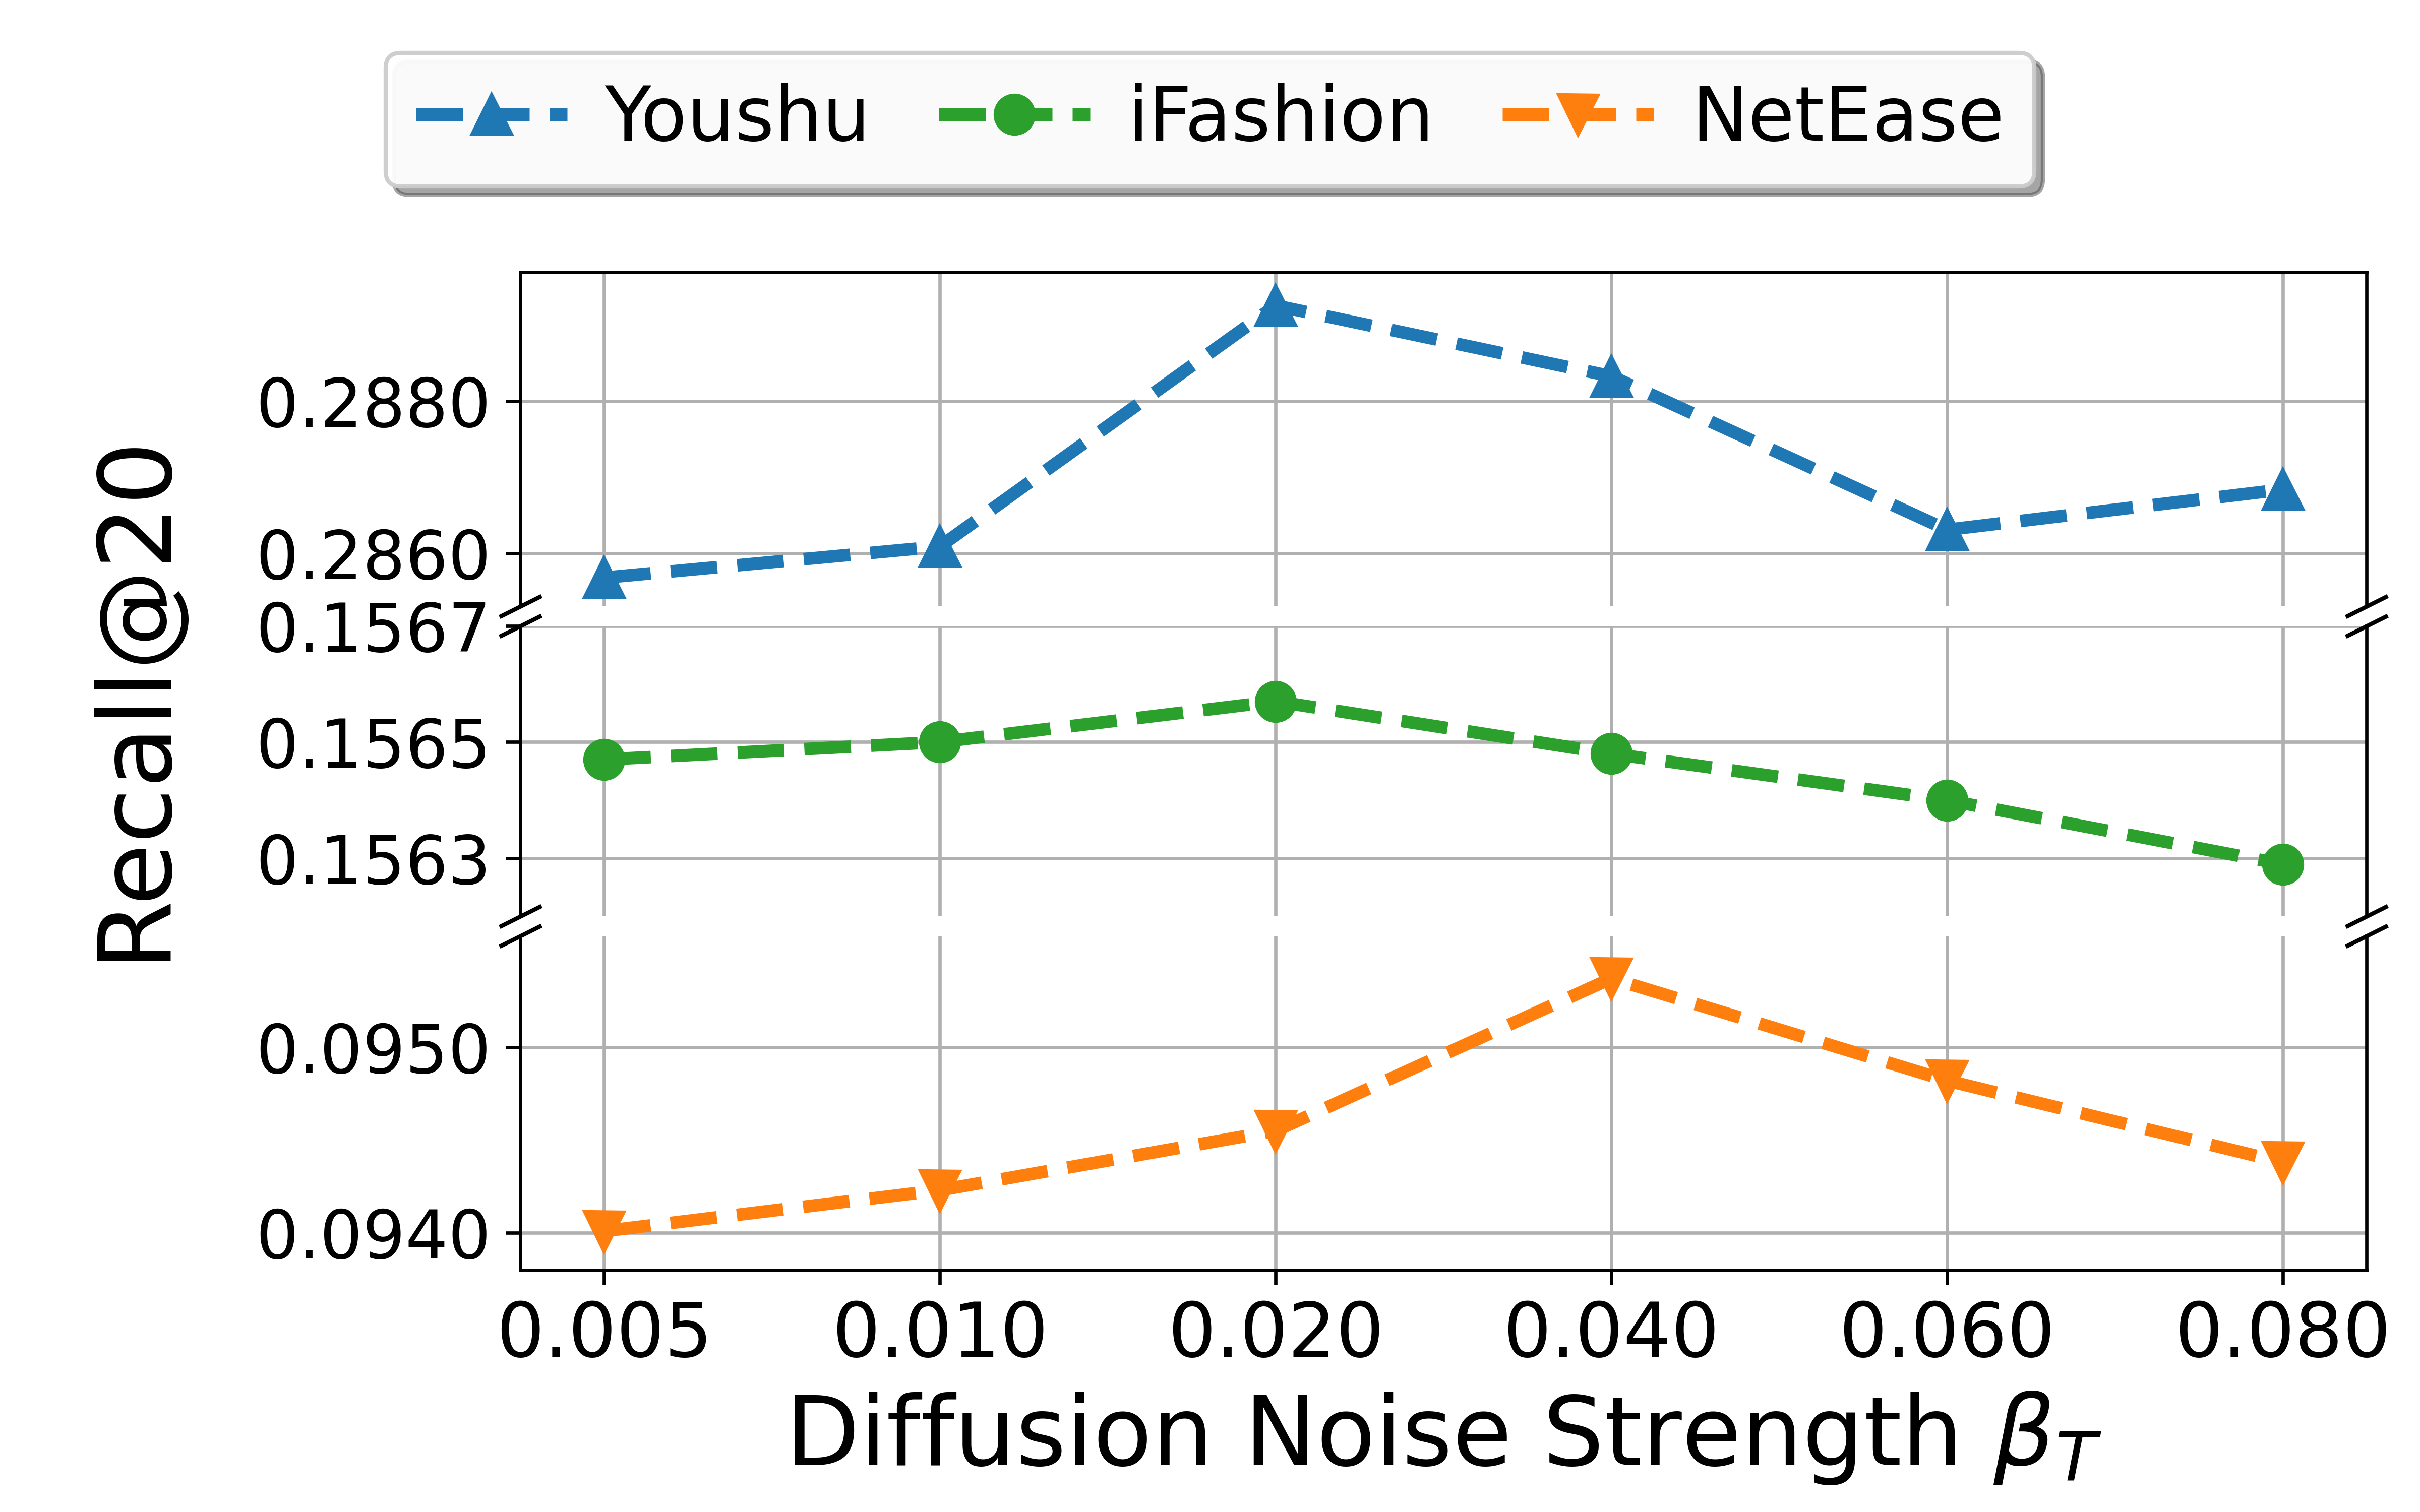
\includegraphics[width=\linewidth]{Figures/hp_betaT.png}
        \vspace{-2pt}
        \centerline{\small (a)}
    \end{minipage}
    \hfill
    \begin{minipage}[t]{0.32\textwidth}
        \centering
        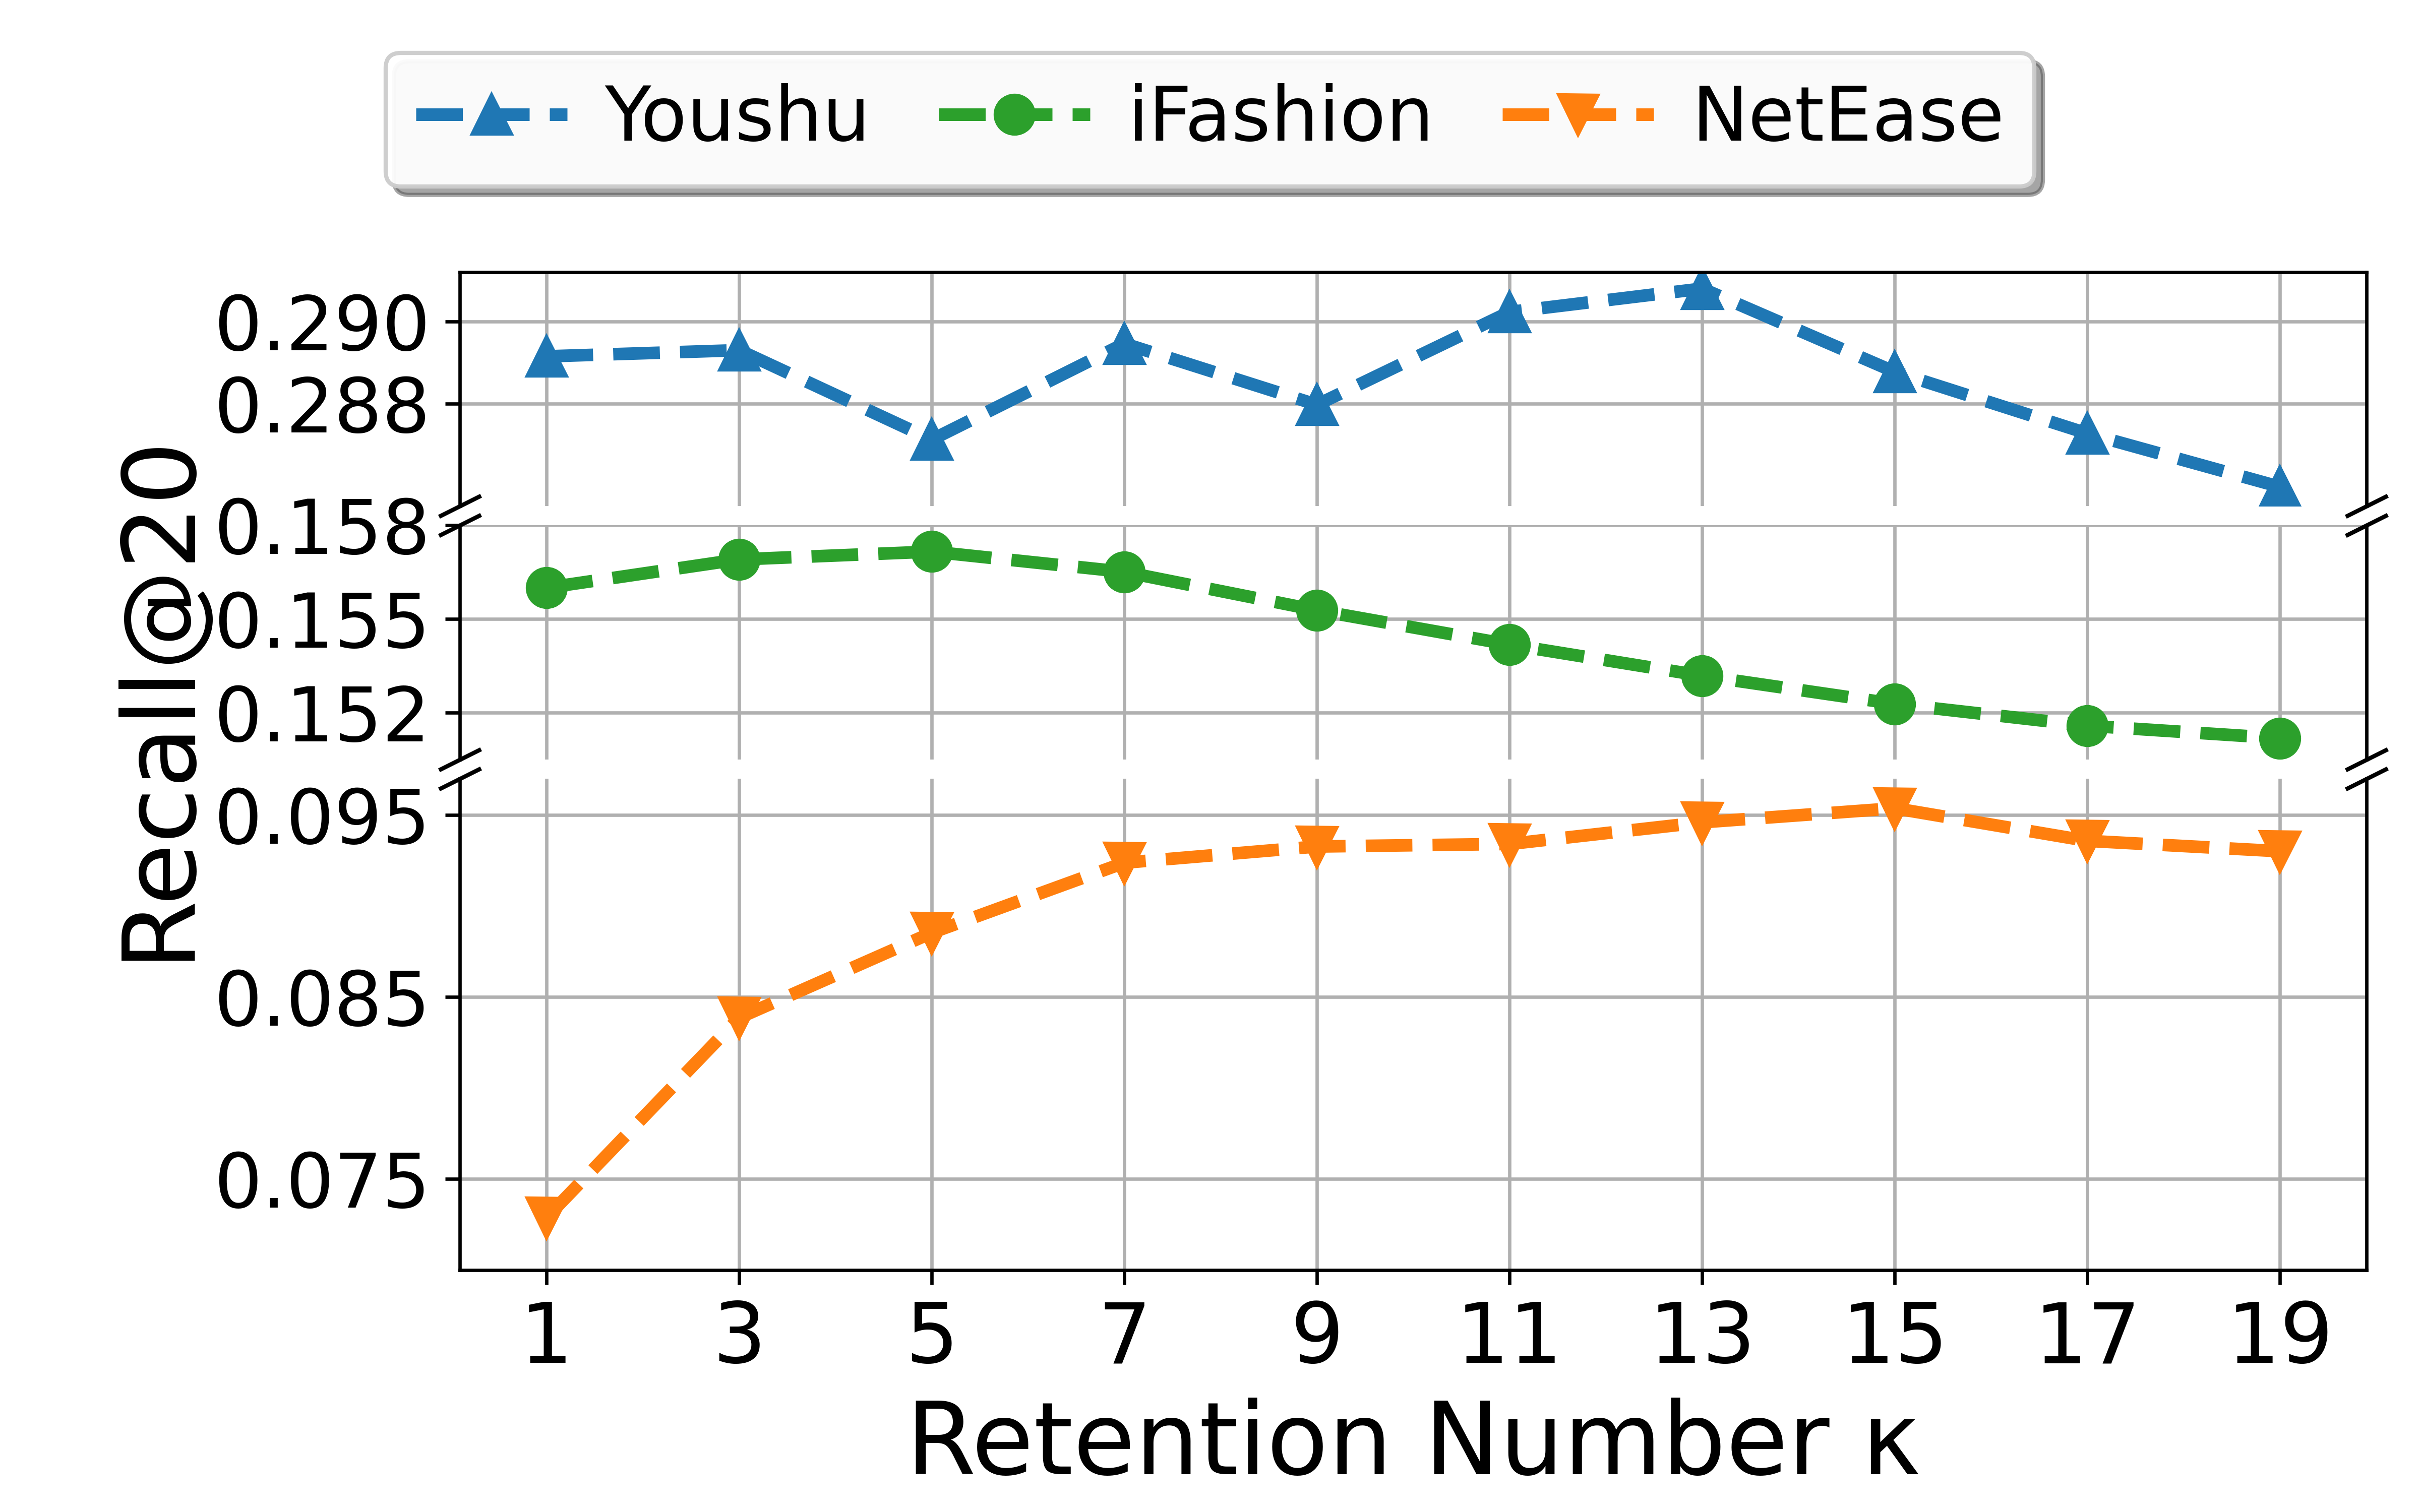
\includegraphics[width=\linewidth]{Figures/hp_kappa.png}
        \vspace{-2pt}
        \centerline{\small (b)}
    \end{minipage}
    \hfill
    \begin{minipage}[t]{0.32\textwidth}
        \centering
        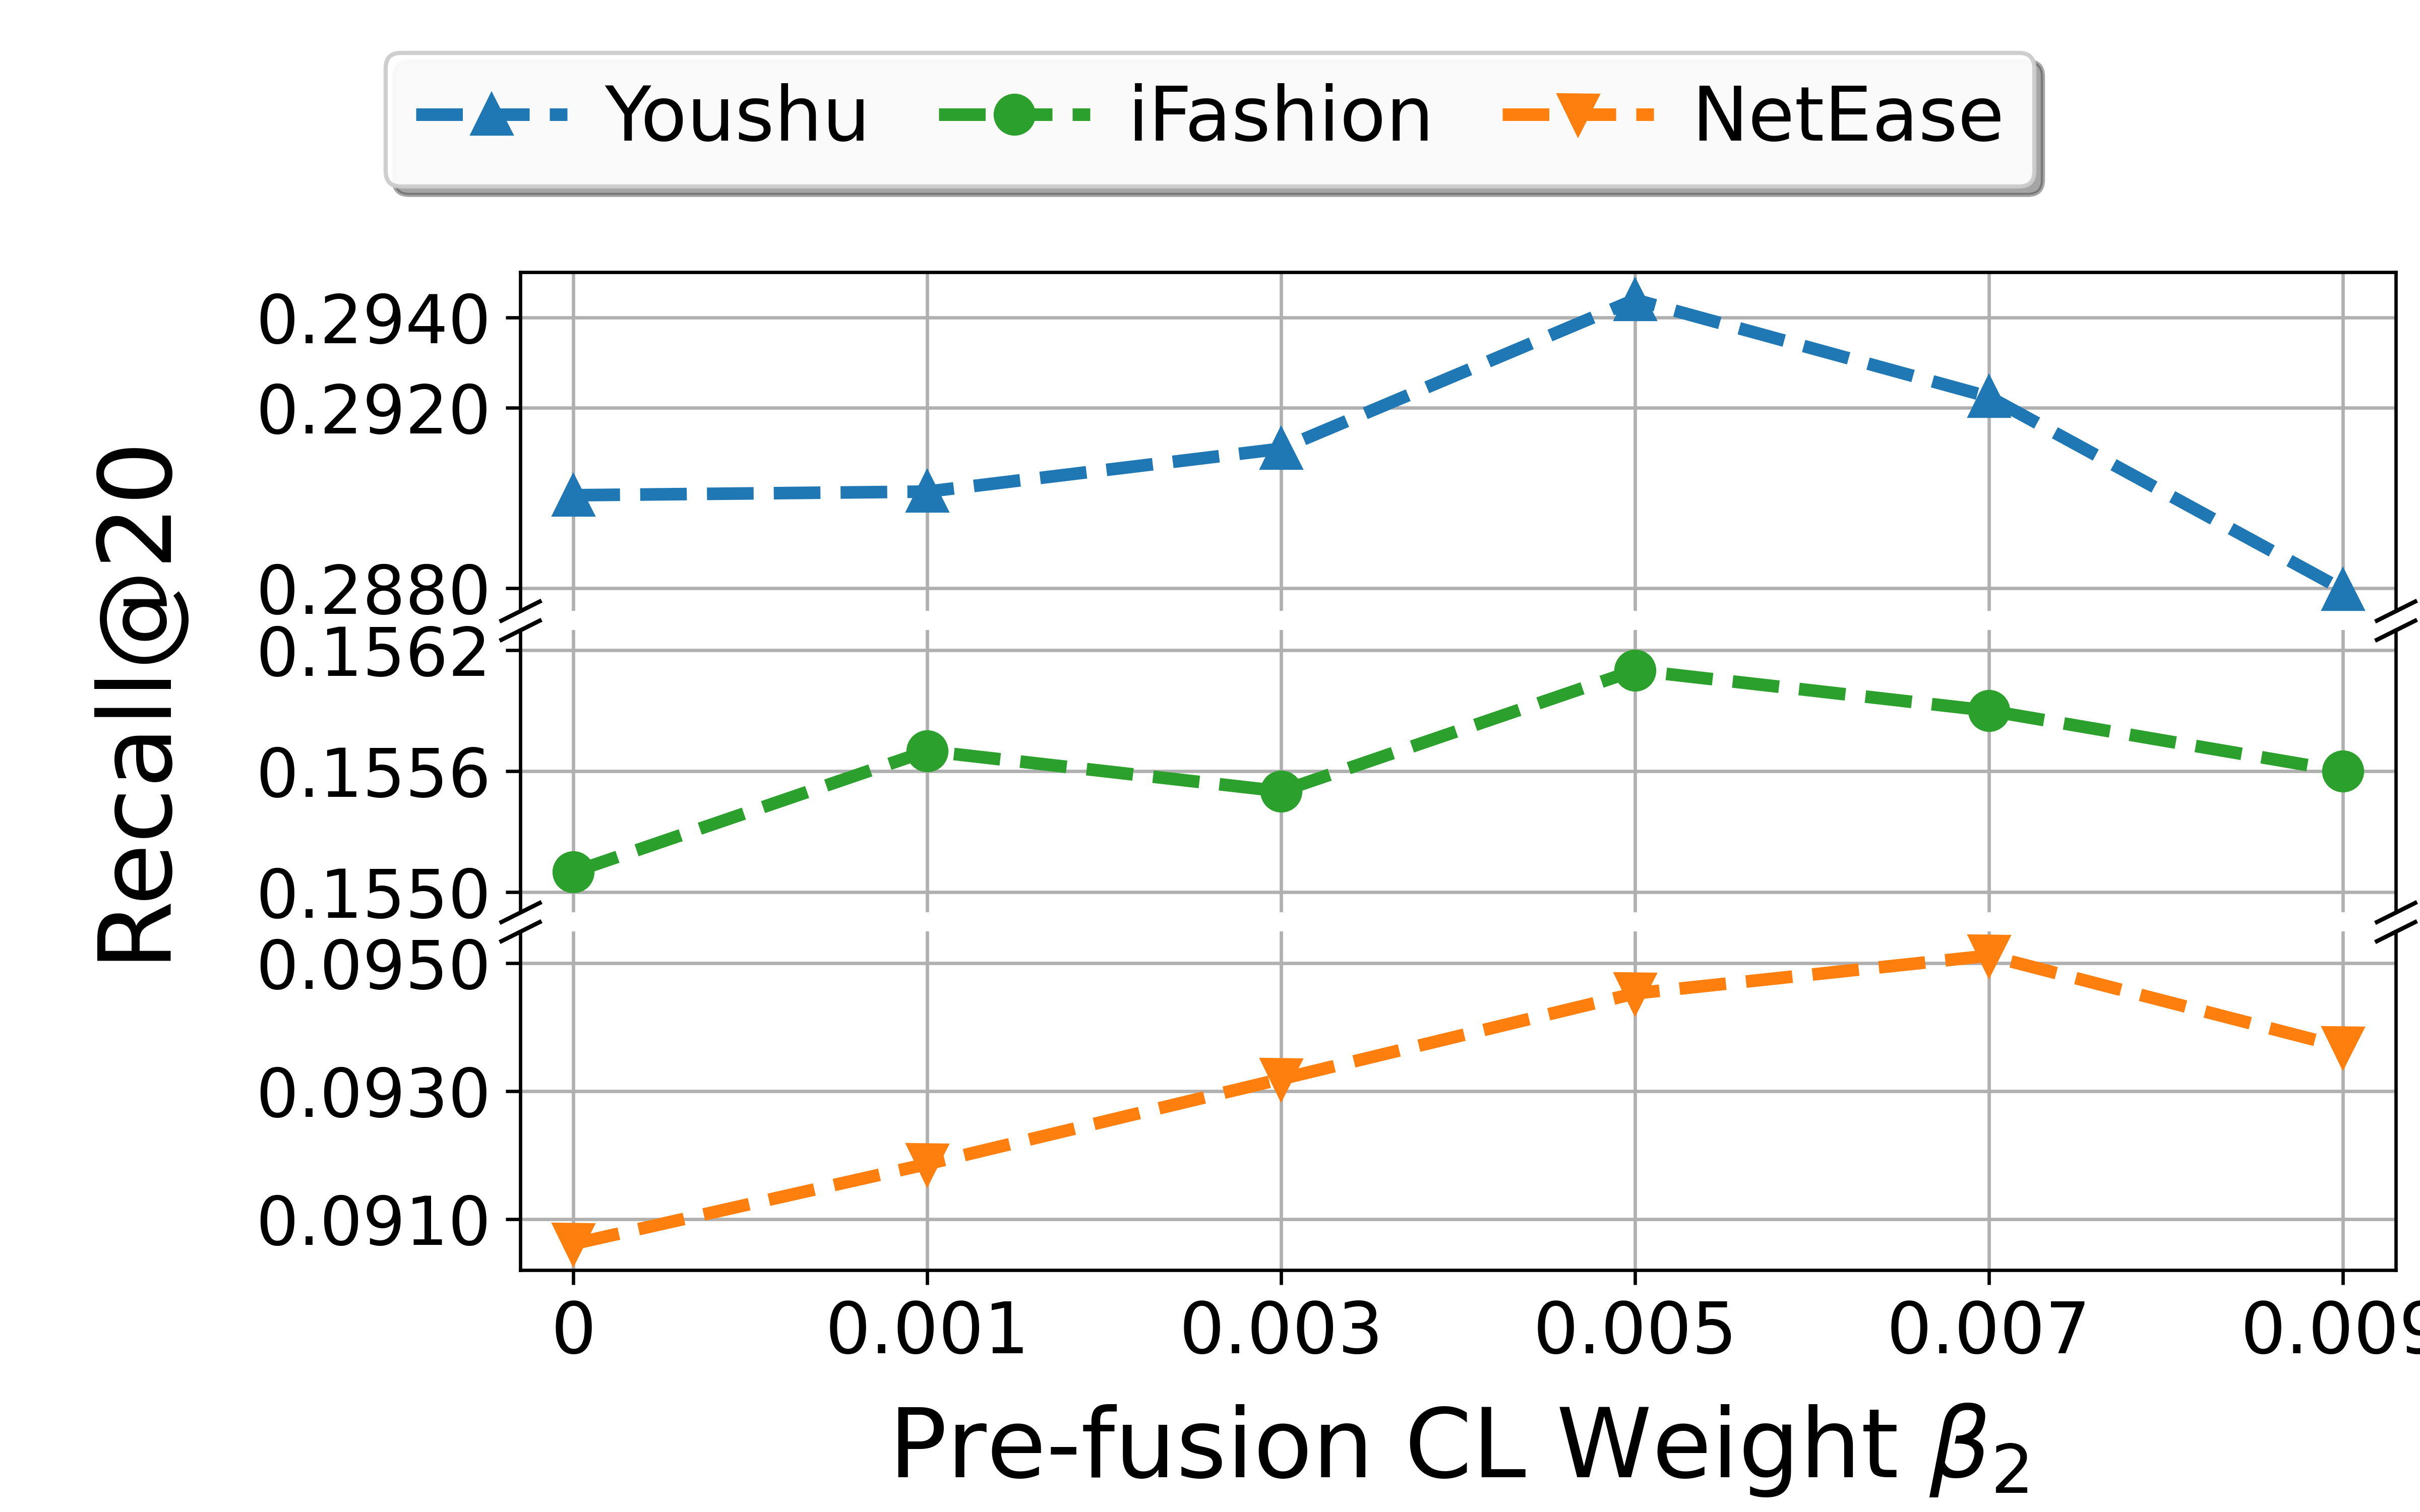
\includegraphics[width=\linewidth]{Figures/hp_beta2.png}
        \vspace{-2pt}
        \centerline{\small (c)}
    \end{minipage}

    \caption{Hyperparameter sensitivity of DiGO on three datasets
    in terms of Recall@20. (a) Diffusion noise strength $\beta_T$,
    which denotes the maximum noise level in the diffusion
    schedule. (b) Retention number $\kappa$ for user--bundle graph
    reconstruction. (c) Weight $\beta_2$ of the pre-fusion
    cross-view contrastive loss. Broken $y$-axes are used to
    accommodate the different performance scales across datasets.}
    \label{fig:hyperparameter}
\end{figure*}


\paragraph{Performance on Sparse Users.}
To investigate whether pre-fusion cross-view contrastive learning
alleviates the limited supervision caused by sparse user--bundle
feedback, we sort users according to their numbers of training
UB interactions and divide them into four equally sized groups.
G1 represents the sparsest users, whereas G4 represents the
densest users. To isolate the effect of pre-fusion contrastive
learning, diffusion-driven graph optimization is disabled in
both compared settings. In
Figure~\ref{fig:in-depth-analysis}(c)--(d),
\textbf{w/o Pre-fusion CL} denotes the multi-view recommendation
backbone without either of the two proposed components, while
\textbf{DiGO} denotes the same setting augmented only with
pre-fusion cross-view contrastive learning. Therefore, the
performance difference between the two variants is solely
attributable to the pre-fusion alignment objective.

Introducing pre-fusion cross-view contrastive learning improves
Recall@20 and NDCG@20 across all four user groups. The largest
gains are observed for the sparsest group G1, where Recall@20
and NDCG@20 increase by 12.64\% and 9.32\%, respectively. The
improvements in the remaining groups are comparatively smaller,
although they do not follow a strictly monotonic pattern. These
results demonstrate that aligning the UI and BI representations
with the UB view is particularly beneficial when direct
bundle-level feedback is severely limited. By transferring
complementary supervision from the two auxiliary relations
before view fusion, the proposed cross-view alignment improves
preference learning for sparse users.





\subsection{Hyperparameter Sensitivity}

We investigate the effects of the diffusion noise strength
$\beta_T$, the retention number $\kappa$, and the pre-fusion
contrastive loss weight $\beta_2$, while varying one
hyperparameter at a time and keeping the others fixed. The
results are shown in Figure~\ref{fig:hyperparameter}.

Moderate values of $\beta_T$ generally yield better
performance, as insufficient noise may provide limited
denoising supervision, whereas excessive noise may obscure
useful preference information. For $\kappa$, retaining too few
interactions removes informative supervision, while retaining
too many may preserve unreliable connections. Similarly, an
appropriate $\beta_2$ improves cross-view alignment, whereas
an overly large value may overemphasize view consistency.
Overall, DiGO maintains stable performance within reasonable
hyperparameter ranges.




\section{Conclusion}

In this paper, we proposed DiGO, a diffusion-driven graph
optimization framework for bundle recommendation. To mitigate
the misleading propagation caused by unreliable interactions in
the user--bundle graph, DiGO models each user's overall bundle
preference through conditional diffusion and uses the resulting
representation to re-evaluate observed interactions and
reconstruct the user--bundle graph for subsequent multi-view
learning. To address the limited supervision caused by sparse
user--bundle feedback, DiGO further uses the reconstructed
user--bundle view as the anchor and aligns the user--item and
bundle--item views before view fusion, thereby supplementing
bundle-level supervision with auxiliary relations. Experiments
on three public datasets demonstrate that DiGO outperforms
existing methods across all evaluation metrics. Ablation studies,
in-depth analyses, and hyperparameter experiments further
validate the effectiveness and robustness of the two key designs.
\end{document}

